\documentclass[a4paper]{article}   	% use "amsart" instead of "article" for AMSLaTeX format
\usepackage[margin=1in]{geometry}
%\documentclass[12pt, oneside]{article}   	% use "amsart" instead of "article" for AMSLaTeX format
\usepackage{textcomp}
\usepackage{geometry}                		% See geometry.pdf to learn the layout options. There are lots.
\geometry{letterpaper}                   		% ... or a4paper or a5paper or ...
%\geometry{landscape}                		% Activate for rotated page geometry
%\usepackage[parfill]{parskip}    		% Activate to begin paragraphs with an empty line rather than an indent
\usepackage{graphicx}				% Use pdf, png, jpg, or eps§ with pdflatex; use eps in DVI mode
\usepackage{caption}
\usepackage{subcaption}								% TeX will automatically convert eps --> pdf in pdflatex
\usepackage{color}
\usepackage{amssymb}
\usepackage{amsthm}
\usepackage{listings}
\usepackage{url}
\newtheorem{theorem}{Theorem}
\newtheorem{definition}{Definition}
\usepackage{natbib}
\usepackage{xcolor}
\usepackage{algpseudocode}
\usepackage{algorithm}
\usepackage{hyperref}


% removed hyperref because of arXiv complaining
\usepackage{authblk}
\usepackage{float}
\usepackage{rotating}
\usepackage{adjustbox}
\usepackage[font=small,labelfont=bf]{caption}
%\usepackage{changes}
\usepackage{changes}
\definechangesauthor[name={George Chacko}, color=blue]{gc}

\renewcommand{\thealgorithm}{S\arabic{algorithm}}
\renewcommand{\thefigure}{S\arabic{figure}}
\renewcommand{\thetable}{S\arabic{table}}
\renewcommand{\thesection}{S\arabic{section}}
\renewcommand{\theequation}{S\arabic{equation}}
\renewcommand{\thetheorem}{S\arabic{theorem}}
\renewcommand{\thelemma}{S\arabic{lemma}}

\hypersetup{
     colorlinks=true,
     linkcolor=blue,
     filecolor=blue,
     citecolor = blue,
     urlcolor=blue,
     }


\usepackage{authblk}
\title{Supplementary Materials for ``Well-Connected Communities in Real-World Networks''}
\author[1]{Minhyuk Park\thanks{Minhyuk Park and Yasamin Tabatabaee contributed equally}}
\author[1]{Yasamin Tabatabaee}
\author[1]{Baqiao Liu}
\author[1]{Vidya Kamath Pailodi\thanks{Vidya Kamath Pailodi and Vikram Ramavarapu contributed equally}}
\author[1]{Vikram Ramavarapu}
\author[1]{Rajiv Ramachandran}
\author[2]{Dmitriy Korobskiy}
\author[3]{Fabio Ayres}
\author[1,4]{George Chacko\thanks{chackoge@illinois.edu}}
\author[1]{Tandy Warnow\thanks{warnow@illinois.edu}}
\affil[1]{Department of Computer Science, University of Illinois Urbana-Champaign, Urbana, IL 61801, USA}
\affil[2]{NTT DATA, McLean, VA 22102, USA}
\affil[3]{Insper Institute, S\={a}o Paulo, Brazil}
\affil[4]{Office of Research, Grainger College of Engineering, University of Illinois Urbana-Champaign, Urbana, IL 61801, USA}


\begin{document}
\maketitle
\tableofcontents
\listoffigures
\listoftables
\newpage


\section{Connectivity Modifier Pipeline}

In this section, we bring the details of each step of the pipeline, in addition to commands. All scripts used for the analysis in this study are available at \href{https://github.com/illinois-or-research-analytics/cm_manuscript/tree/main/analysis}{https://github.com/illinois-or-research-analytics/cm\_manuscript/tree/main/analysis}, and the CM code is available at \href{https://github.com/RuneBlaze/connectivity-modifier}{https://github.com/RuneBlaze/connectivity-modifier}.

\subsubsection*{Preprocessing the network}
Before running the CM pipeline, we removed duplicate/parallel edges and self-loops from the networks, using the \texttt{cleanup\_el.R} script with the following command:

\begin{lstlisting}[basicstyle=\ttfamily\small]
Rscript cleanup_el.R <original_network.tsv> <cleaned_network.tsv>
\end{lstlisting}

\subsubsection*{CM Pipeline}
The cleaned input network $\mathcal{G}$ is then processed in a pipeline that has the following stages:
\begin{itemize}
\item \textbf{Clustering}: Clustering $\mathcal{G}$, using either the Leiden algorithm (in default mode with two iterations) or Iterative K-core Clustering (IKC) method, with the following commands respectively:

\begin{lstlisting}[basicstyle=\ttfamily\small]
leidenalg.find_partition(net, leidenalg.CPMVertexPartition, resolution_parameter=r)
\end{lstlisting}

\begin{lstlisting}[basicstyle=\ttfamily\small]
IKC.py -e <cleaned_network.tsv> -k 10 -o <output file>
\end{lstlisting}

We used the Python version of Leiden (leidenalg v0.8.2) available at \href{https://github.com/vtraag/leidenalg}{https://github.com/vtraag/leidenalg} and IKC (v1.0.0) available at \href{https://github.com/chackoge/ERNIE_Plus/blob/master/Illinois/clustering/eleanor/code/IKC.py}{https://github.com/chackoge/ERNIE\_Plus/blob/master/Illinois/clustering/} \href{https://github.com/chackoge/ERNIE_Plus/blob/master/Illinois/clustering/eleanor/code/IKC.py}{eleanor/code/IKC.py}.


\item  \textbf{Filtering}: Removing clusters of size less than or equal to 10 as well as trees (defined as connected clusters where the number $m$ of edges is one less than the number $n$ of vertices, i.e. $m=n-1$).
%Depending on the user and the dataset being analyzed, one of the following options was used to perform this step: \textcolor{red}{just write one option that should be used}
%\begin{enumerate}
%\item \texttt{belinda} \citep{belinda2022} expressions, e.g., \texttt{g1.filter(pl.col('n') > 10)} and %\texttt{g1.filter(pl.col('n') != pl.col('m') + 1)}
%\item \texttt{find\_trees.py}: a slow script that relies on Networkit \citep{Staudt2016}
%\item \texttt{cluster\_analyzer.py}: a parallelized version of find\_trees.py
%\item \texttt{subset\_graph\_nonnetworkit.R}: a fast script without dependence on Networkit that also returns maxDegree for a cluster.
%\end{enumerate}
\item  \textbf{CM}: Applying connectivity modifier, available at \href{https://github.com/RuneBlaze/connectivity-modifier}{https://github.com/RuneBlaze/connectivity-modifier} with the following commands (assuming the clustering method used is Leiden), where the option \texttt{-g} specifies the resolution parameter:
\begin{lstlisting}[basicstyle=\ttfamily\small]
$ cm -i <cleaned_network.tsv> -c leiden -e <filtered_leiden_clustering.tsv> -g <r>
-t 1log10 -o <cm_output.tsv>
$ cm2universal -g <cleaned_network.tsv> -i <cm_output.tsv> -o <cm_output.tsv>
\end{lstlisting}
\item \textbf{Filtering}: Removing clusters of size at most 10  (note: there will not be any trees left at this point) using the same commands as the first filtering step.
\end{itemize}



\section{Pseudocode for the Connectivity Modifier}
\textcolor{red}{this section can be merged with the previous one}
The input to the Connectivity Modifier (CM) is a network and a  clustering; the output will be a set of well-connected clusters (WCC), obtained
by processing each cluster in the input.
Thus, each cluster in the output WCC will be a subset of one of the input clusters.
Here we describe CM, beginning  with the necessary definitions.

\begin{itemize}
    \item $\delta(C)$: the minimum degree of  any node in cluster $C$
    \item $deg(u)$: the degree of node $u$
    \item $t(C)$: minimum required edge cut size for  $C$
    \item $\lambda(C)$: the minimum edge cut size of $C$
    \item $mod(C, H)$: modularity of subgraph $H$ w.r.t.~$C$
    \item $f$: clustering method: a clustering method takes as input a graph, and outputs non-singleton subgraphs of the input graph.
\end{itemize}

Recall that  $t(C)$ is the {\em smallest} cut that can still be considered ``large enough".
Furthermore, in our experiments, we set $t(C) = \lfloor \log_{10}(n) \rfloor +1$.  This means that any cut that is below $t(C)$ in a number of vertices
will be considered small, and so will be cut.
Here we explore the effect of this definition of $t(C)$, where $C$ is a cluster with $n$ vertices.
\begin{itemize}
\item
$1 \leq n \leq 9$.
For all values of $n$ in this range, we obtain $t(C) = \lfloor log_{10}(n) \rfloor +1$, and so $t(C) = 1$.  Hence, for $1 \leq n \leq 9$, we  only require that the
cluster be connected.
\item
$10 \leq n \leq 99$. For all values of $n$ in this range, we have
 $t(C) = 2$, which means that if $C$ is a cluster of size $n$ and it has a cut of size $1$, that  cut will
be considered ``too small", and will be cut.  Effectively this only ensures that clusters of size between $10$ and $99$ do not have cut edges.
If a cut edge is found, it will mean that in the CM code, that cut edge will be deleted, thus separating the cluster into two pieces.
In contrast, a cut of size $2$ will be considered large enough, and will not be cut.
\item
$100 \leq n \leq 999$.
For all values of $n$ in this range, we have $t(C)=3$, which means that if $C$ has a cut of size  at most $2$ it will be considered
too small, and any such cut will be deleted from $C$.
In contrast, a cut of size $3$  or larger will be considered large enough, and will not be cut.
\item
$1000 \leq n \leq 9999$.
For all values of $n$ in this range, we have $t(C)=4$, which means that if $C$ has a cut of size $3$ or smaller it will be considered
too small, and any such cut will be deleted from $C$.
In contrast, a cut of size $4$ or larger will be considered large enough, and will not be cut.
\end{itemize}

\clearpage
\begin{algorithm}[h]
\caption{Pseudocode for min-cut validity pipeline. The input is a network $\mathcal{G}$ with $N$ vertices and a clustering method $f$ (e.g. Leiden, IKC), and the output is a set of well-connected clusters WCC.}
\begin{algorithmic}[2]
\State $f$: Clustering method (e.g., IKC, Leiden, etc.)
\Function{$g$}{$\mathcal{G}$}
\State WCC $\gets []$ \Comment{This is an empty array}

\State clusters $\gets f(\mathcal{G})$ \Comment{This is an array of clusters generated by $f$}
\State stack $\gets$ clusters
\While{!stack.empty()} \Comment{While there is a cluster in the stack}
    \State $H$ = stack.pop()
    \While{$\delta(H) < t(H)$}
    \State delete an arbitrary node $u$ from $H$ where $deg(u) = \delta(H)$
    \EndWhile
    \If{$\lambda(H) < t(H)$} \Comment{If the edge cut for H is smaller than $t$}
        \State $H_a, H_b$ $\gets$ $H$ separated by a minimum cut
        \State stack.extend($f(H_a)$) \Comment{Recluster $H_a$ and $H_b$}
        \State stack.extend($f(H_b)$)  \Comment{and add clusters to stack}
    \Else
       % \If{$f$ is not modified IKC $\lor$ $mod(G, H) \ge 0$}
            \State WCC $\gets$ WCC $+$ [$H$] \Comment{Add H to WCC}
        \EndIf
\EndWhile
%\If{$f = $ IKC}
%    \State remove all clusters from ans that have modularity $\leq 0$
%    \EndIf
%\textcolor{blue}{}
\State \Return WCC \Comment{WCC contains only well-connected clusters}
\EndFunction
\end{algorithmic}

\label{alg:full-pipeline}
\end{algorithm}

\textbf{Note:} When
$f$ (the clustering method) is IKC, we have made a small modification to the
code for the sake of efficiency.
Specifically, IKC requires that all the clusters have positive modularity.
 In our CM code, the recursive
calls to the clustering method (IKC) in lines 13 and 14 do not check for positive modularity; instead, this check is delayed until the stack is empty (i.e., after line 18).
At this point, it is possible that some of the clusters in WCC will not have positive modularity.
Therefore, when we run CM with IKC for the clustering method $f$,  we add a processing step after line 18 that checks each cluster in WCC for positive modularity,
and deletes any cluster that fails this test.
Only after pruning all such clusters from WCC will we return what is left.

\clearpage
\section{Emulating Real Networks with LFR Graphs}

\textcolor{red}{write the math behind fitting power-law, table with network properties, plots comparing degree distribution and community size distribution of networks vs lFR graphs, commands for generating LFRs, runtime, that we had to change the range of cluster sizes to enable it to generate the network., LFR is not robust to changes in parameters}

\begin{figure}[H]
\centering
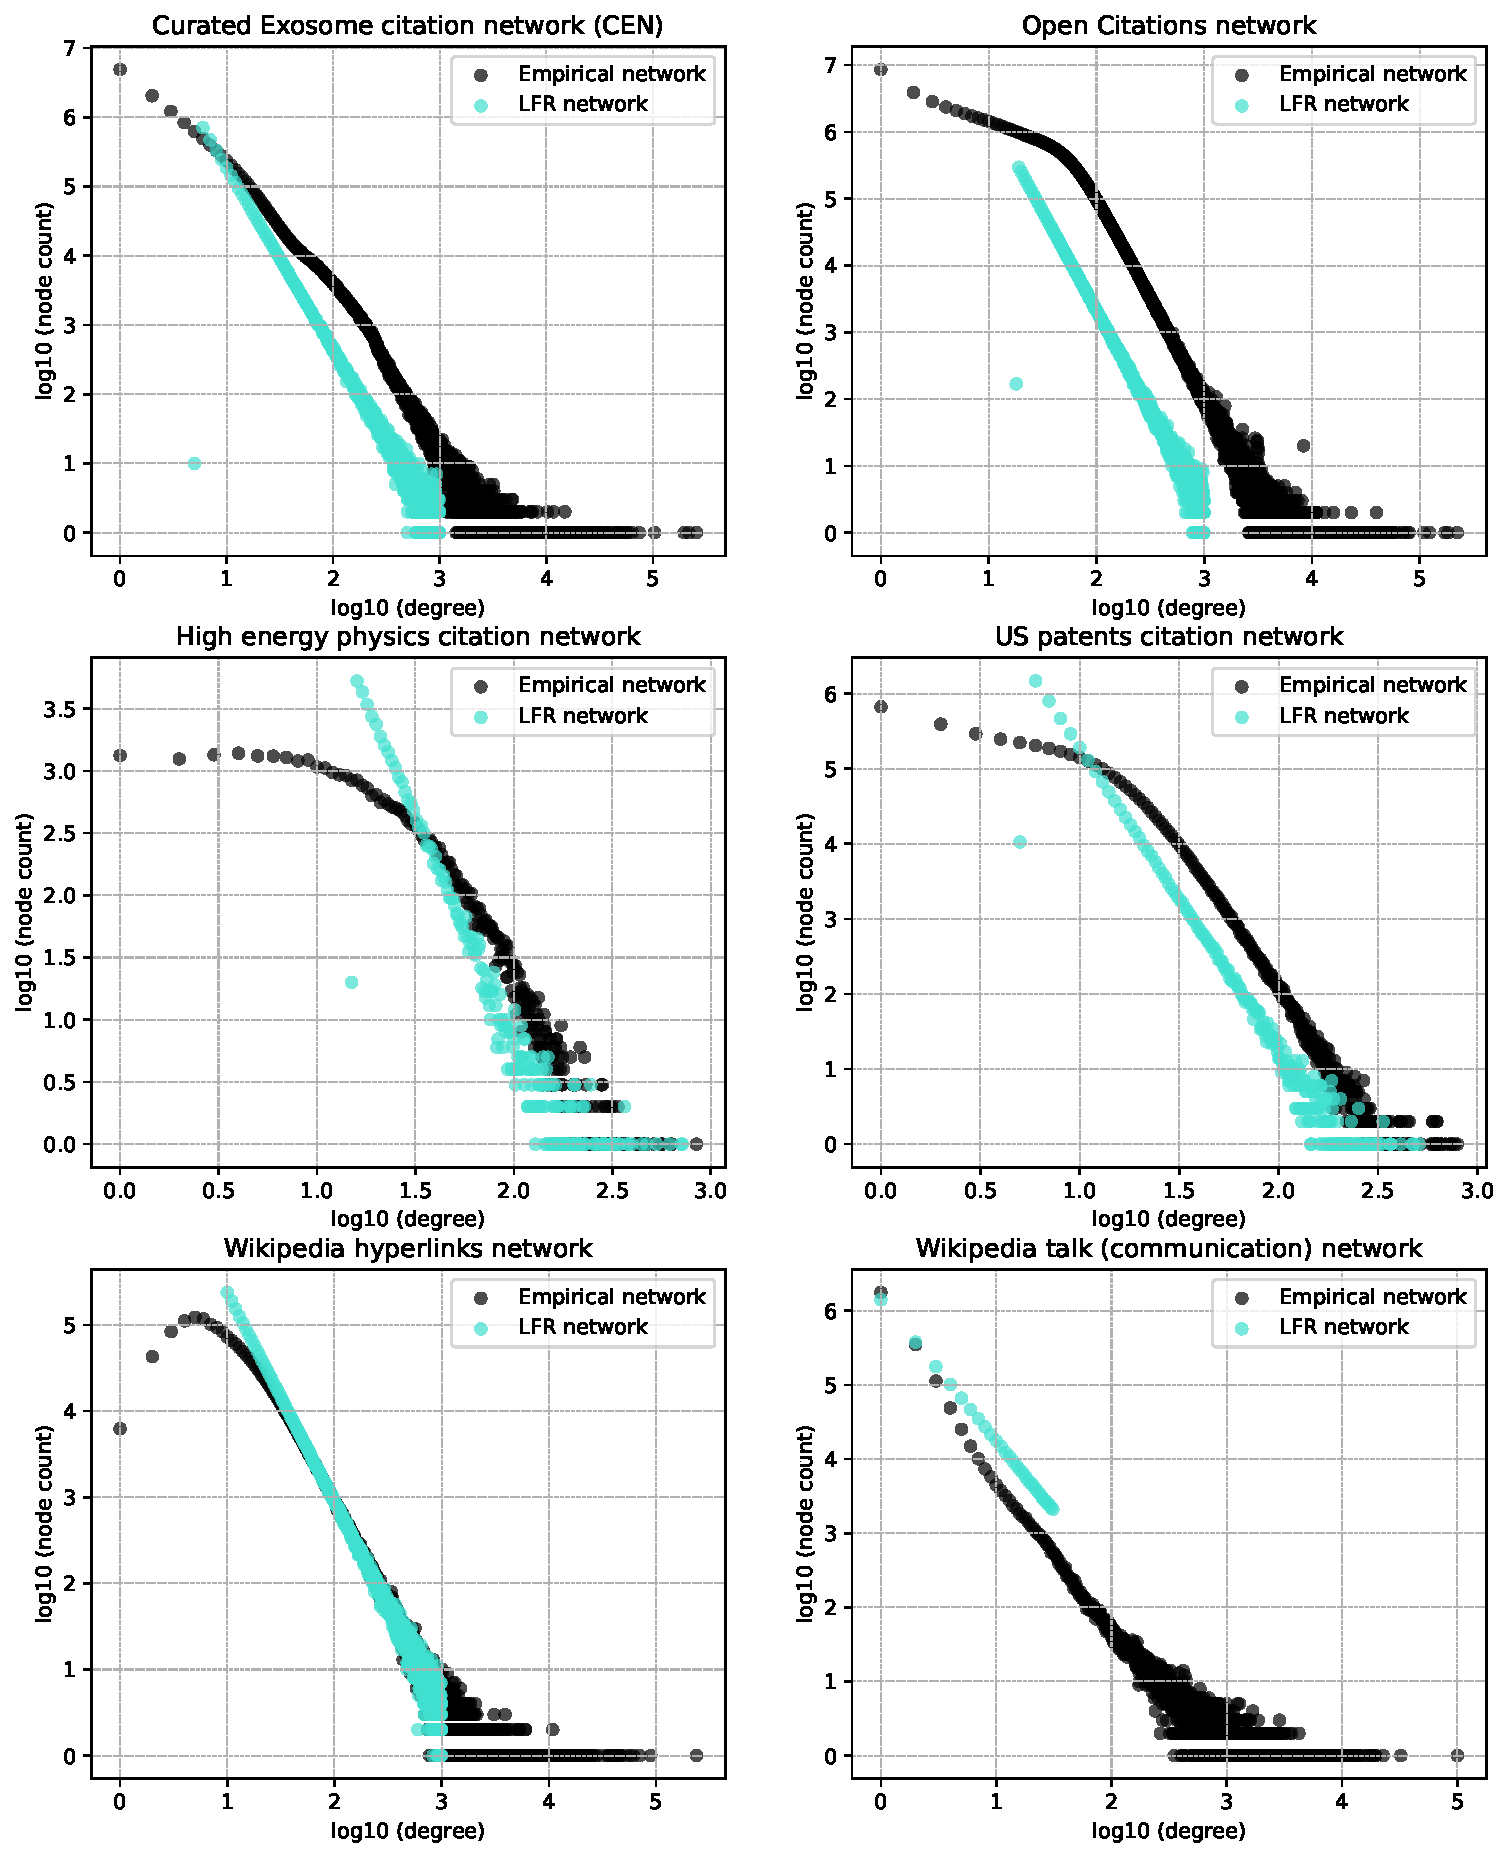
\includegraphics[width=0.85\linewidth]{figs/all_degrees.pdf}
\caption[Comparison between the degree distribution of empirical and LFR networks.]{\textbf{Comparison between the degree distribution of empirical and LFR networks.} The LFR networks are produced to emulate the characteristics of their corresponding real network. For the CEN and the OpenCitations network, the number of nodes of the LFR network is 3,000,000, and for the other networks it exactly matches the number of nodes in its corresponding empirical network. The resolution parameter used for generating the LFR graphs shown in this figure is 0.1. }
\end{figure}

\begin{figure}[H]
\centering
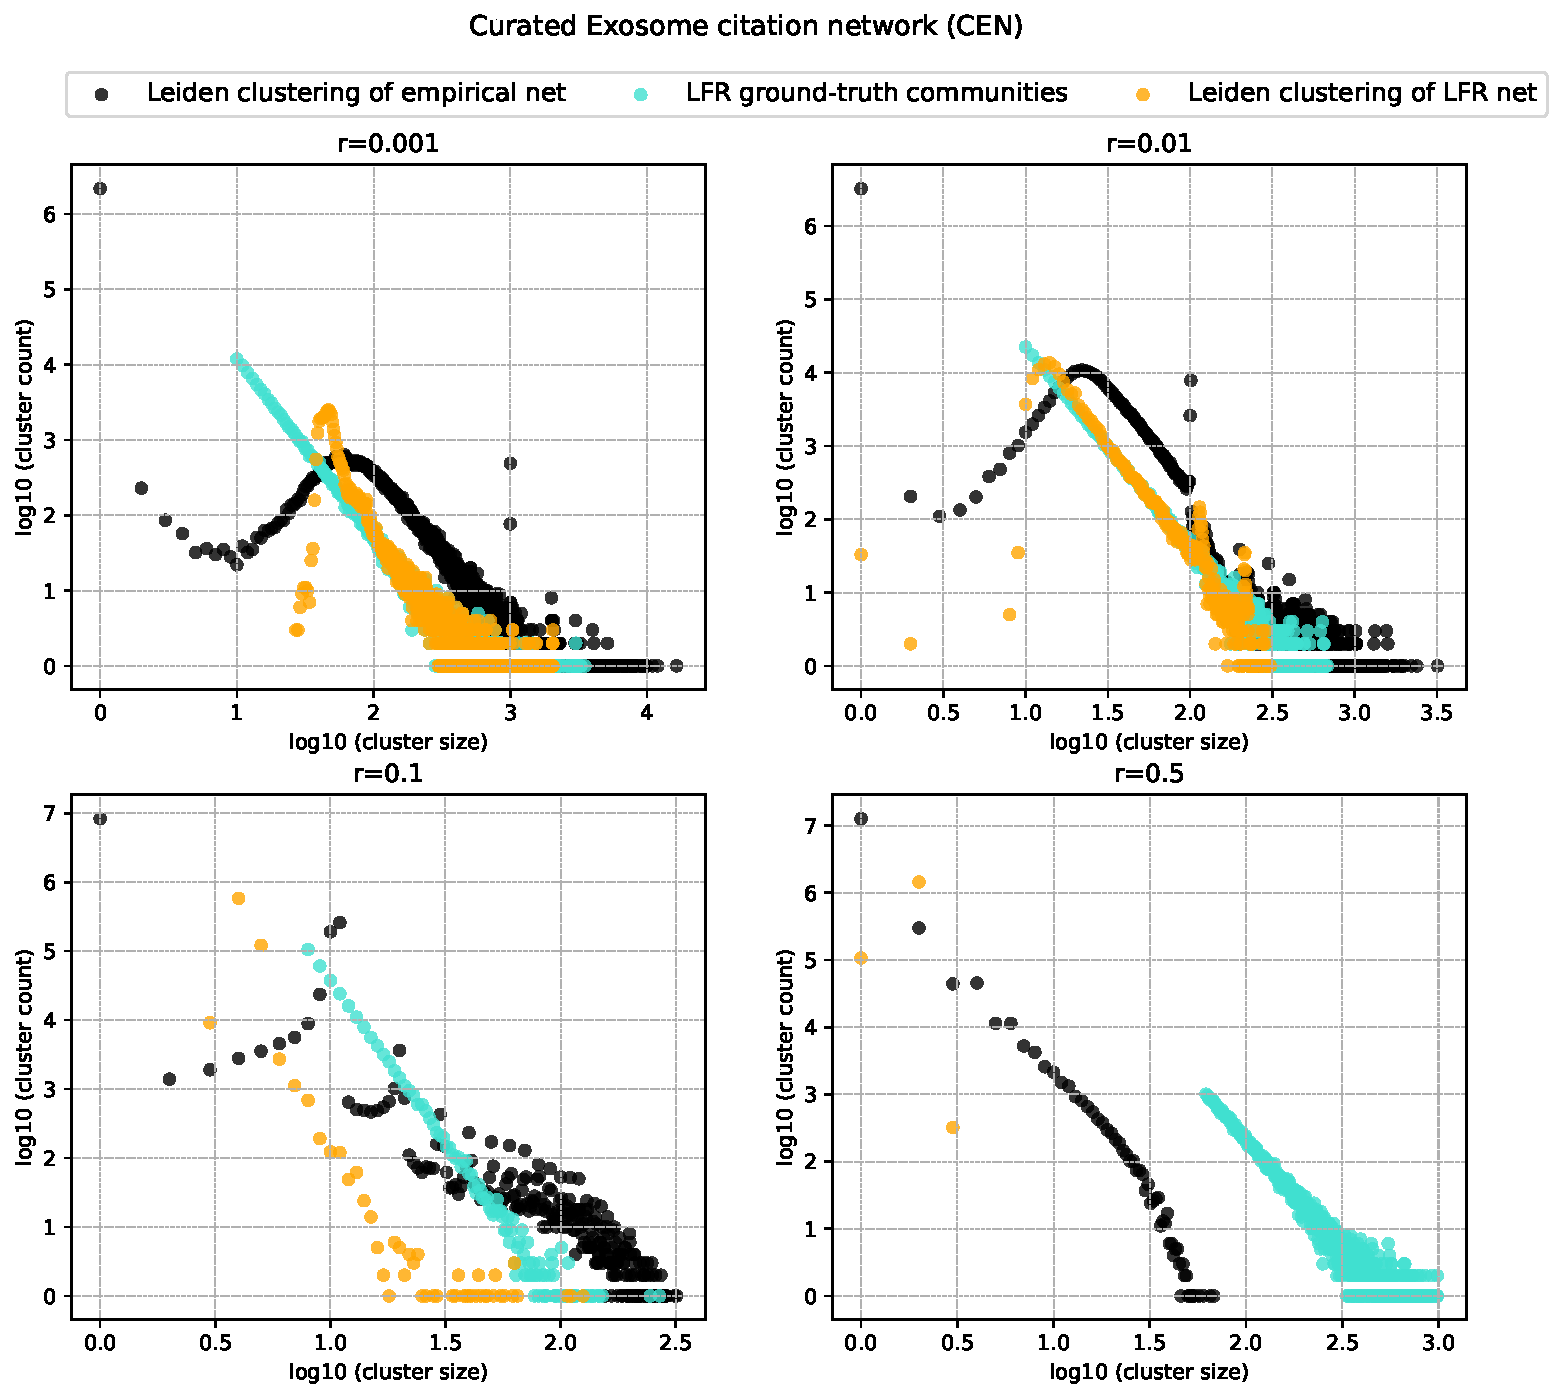
\includegraphics[width=0.85\linewidth]{figs/cen_cm_size.pdf}
\caption[Cluster size distribution for CEN citation networks.]{\textbf{Cluster size distribution for CEN citation networks.} The LFR ground-truth communities (shown in green) are generated according to the parameters estimated from the Leiden clustering of the empirical network (in black), and then the LFR network is re-clustered using Leiden with the same resolution value. }
\end{figure}

\begin{figure}[H]
\centering
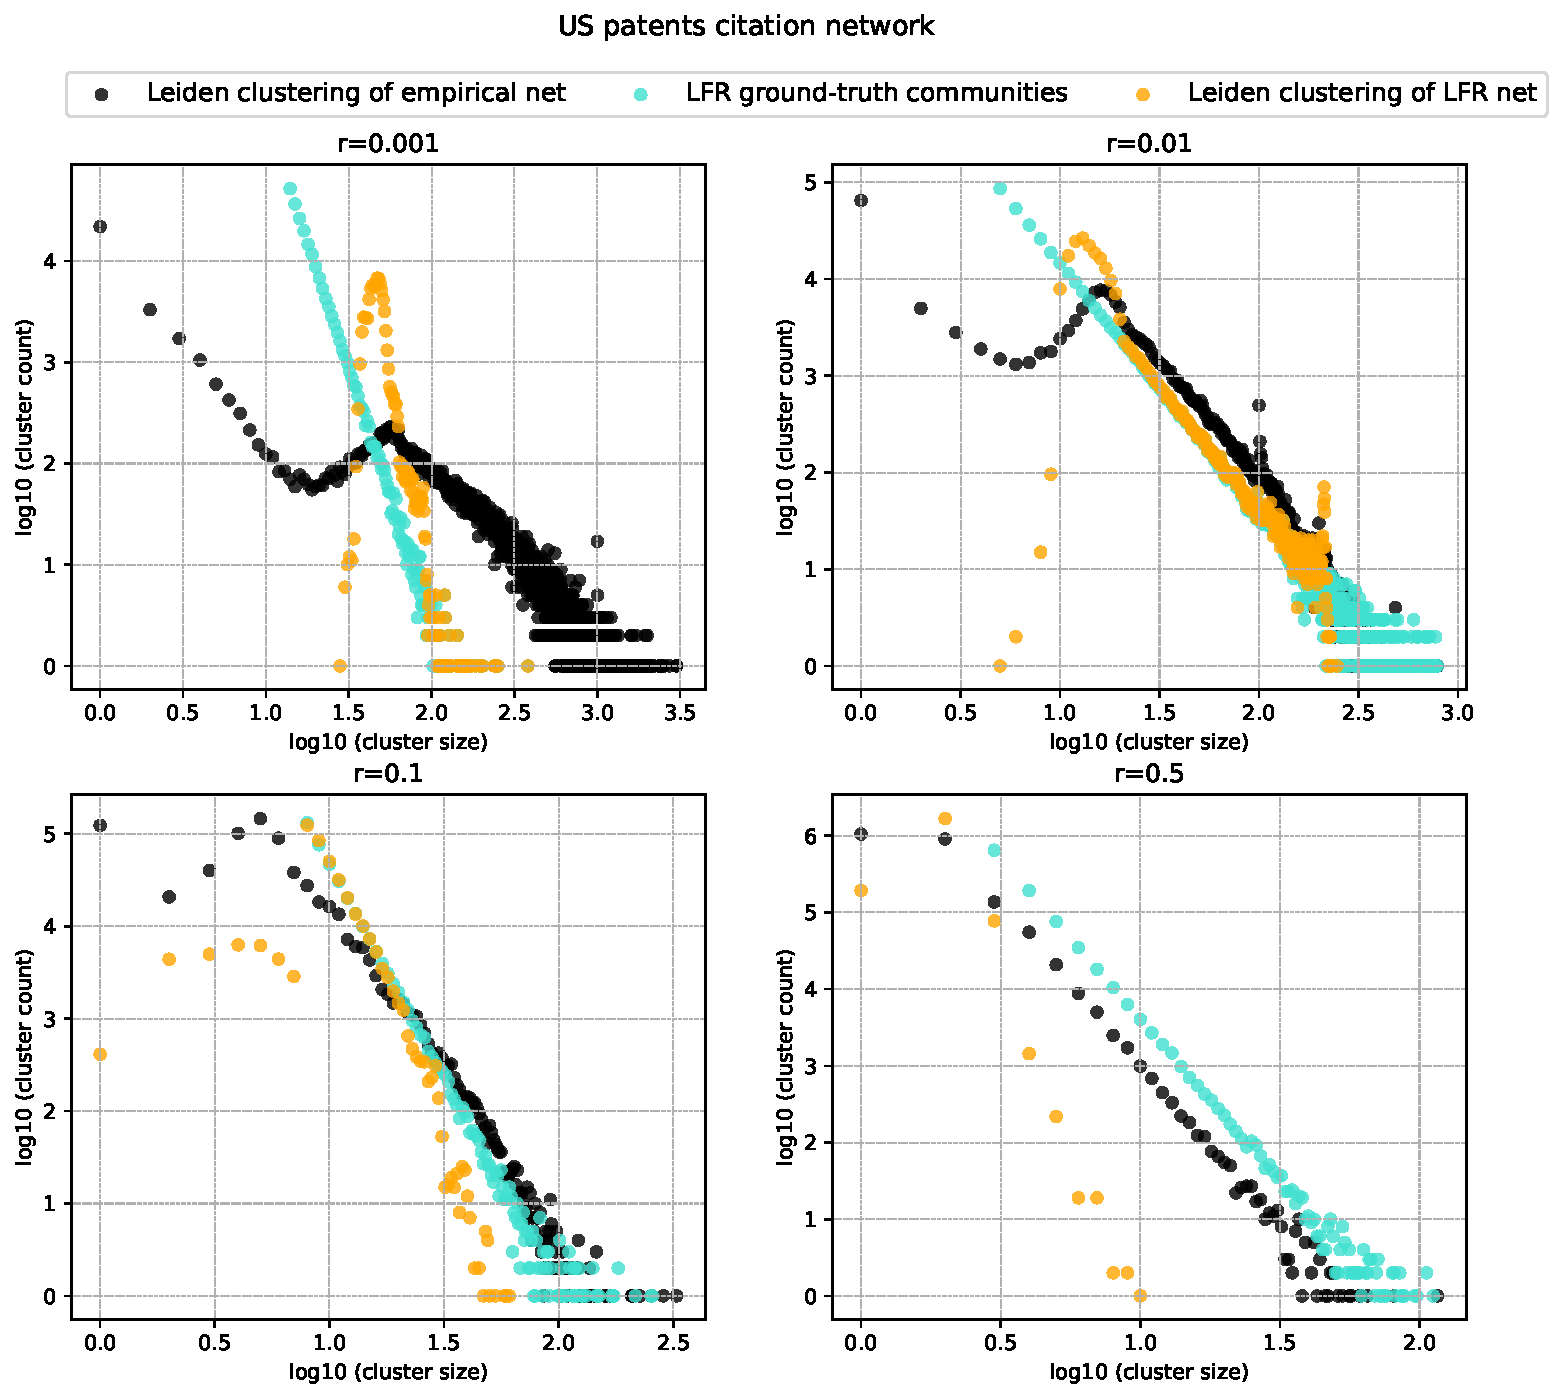
\includegraphics[width=0.85\linewidth]{figs/cit_patents_cm_size.pdf}
\caption[Cluster size distribution for US patents citation networks.]{\textbf{Cluster size distribution for US patents citation networks.} The LFR ground-truth communities (shown in green) are generated according to the parameters estimated from the Leiden clustering of the empirical network (in black), and then the LFR network is re-clustered using Leiden with the same resolution value. }
\end{figure}

\begin{figure}[H]
\centering
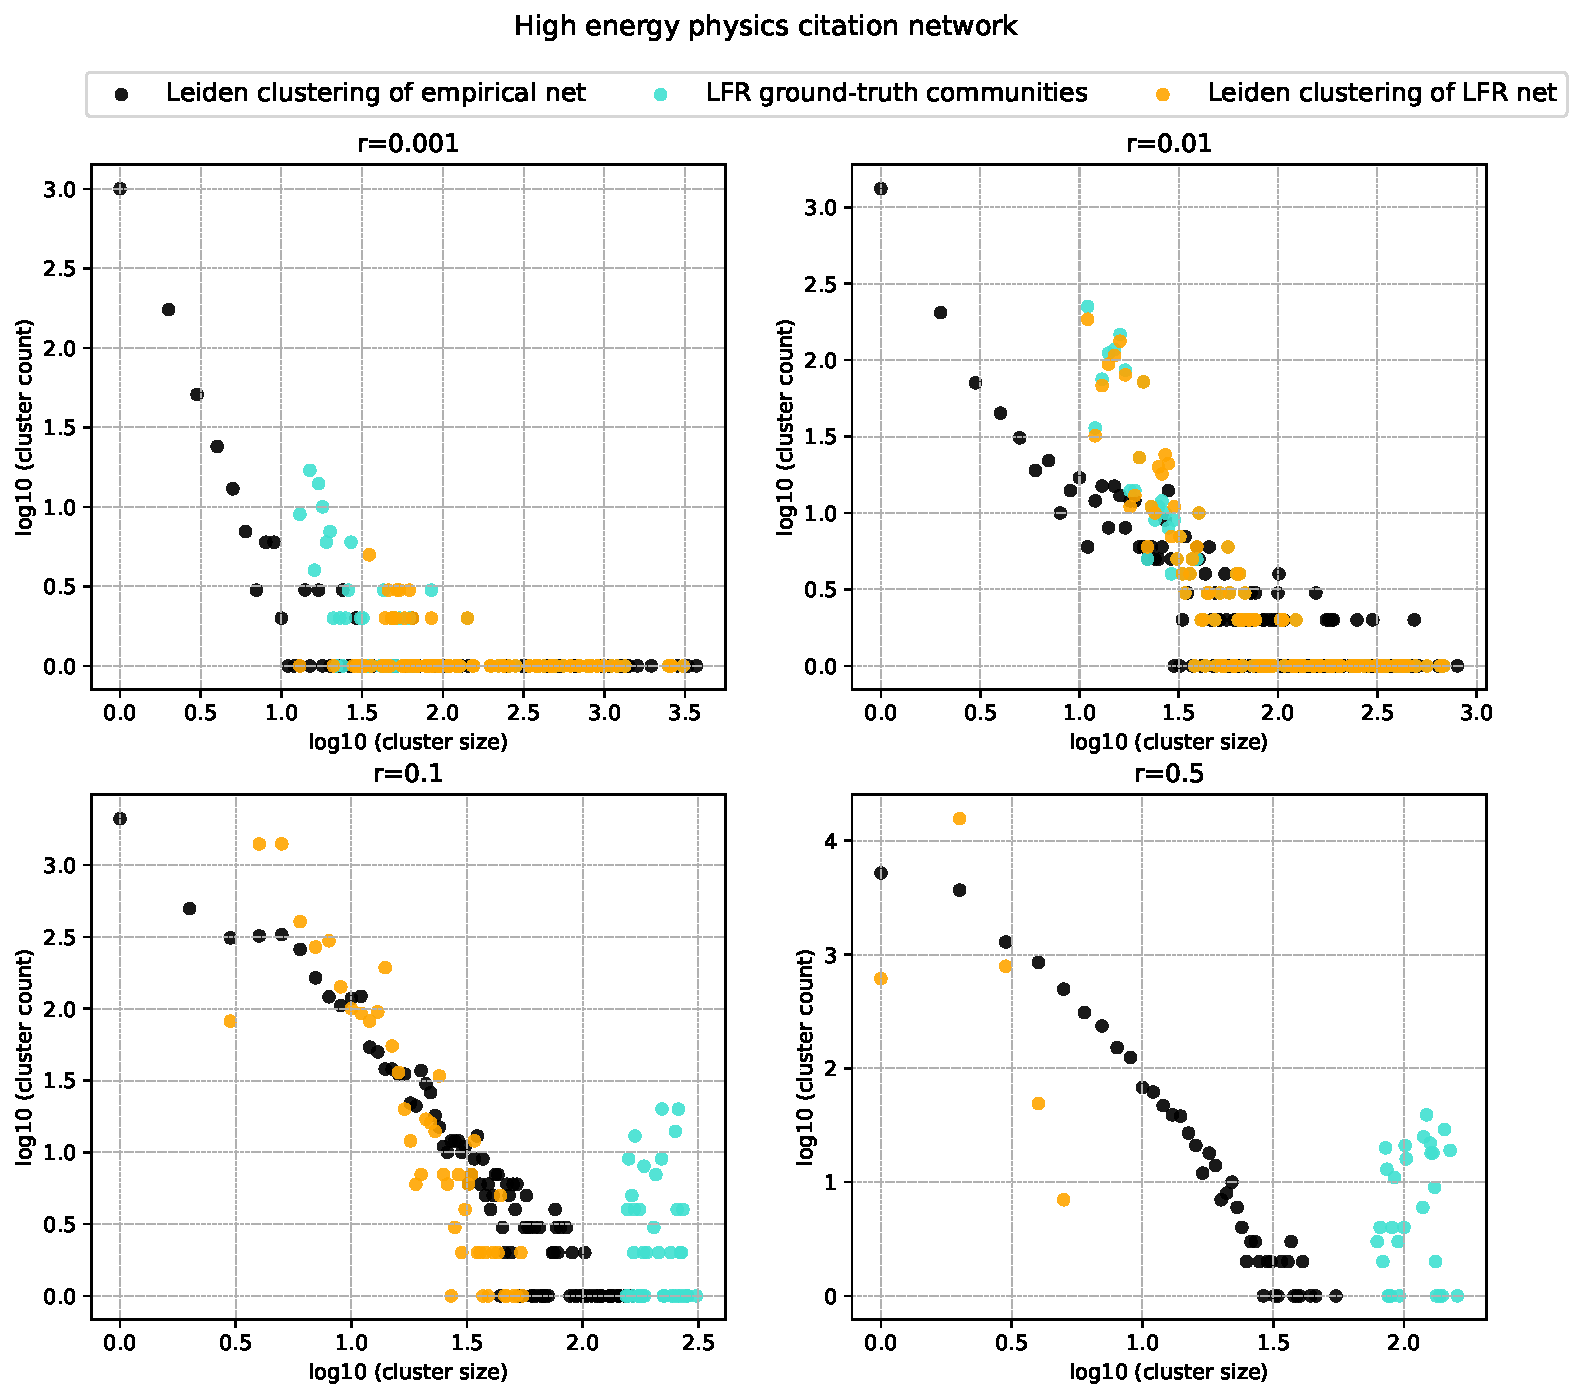
\includegraphics[width=0.85\linewidth]{figs/cit_hepph_cm_size.pdf}
\caption[Cluster size distribution for High Energy physics citation networks.]{\textbf{Cluster size distribution for High Energy physics citation networks.} The LFR ground-truth communities (shown in green) are generated according to the parameters estimated from the Leiden clustering of the empirical network (in black), and then the LFR network is re-clustered using Leiden with the same resolution value. }
\end{figure}


\begin{figure}[H]
\centering
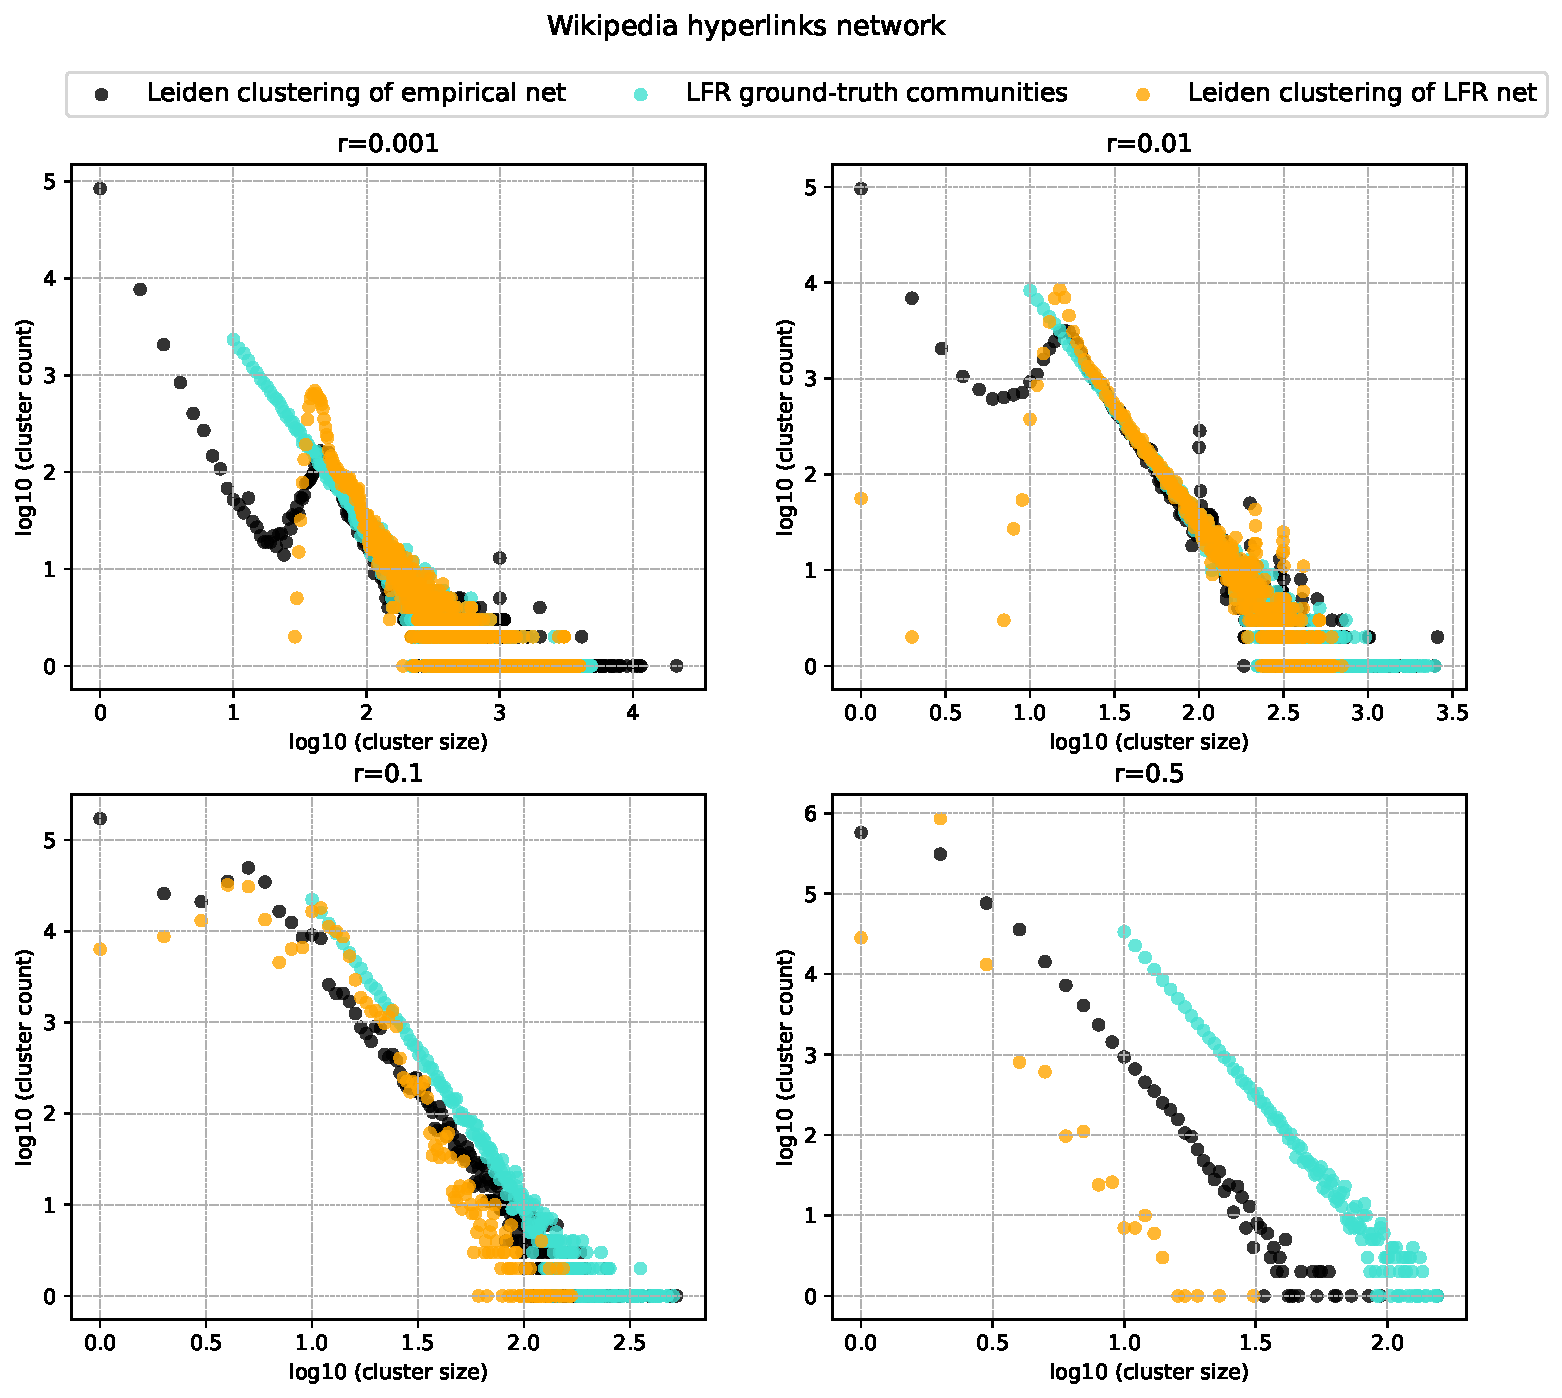
\includegraphics[width=0.85\linewidth]{figs/wiki_topcats_cm_size.pdf}
\caption[Cluster size distribution for Wikipedia hyperlink networks.]{\textbf{Cluster size distribution for Wikipedia hyperlink networks.} The LFR ground-truth communities (shown in green) are generated according to the parameters estimated from the Leiden clustering of the empirical network (in black), and then the LFR network is re-clustered using Leiden with the same resolution value. }
\end{figure}

\section{Additional Results for the CM pipeline}

\begin{figure}[h!]
\centering
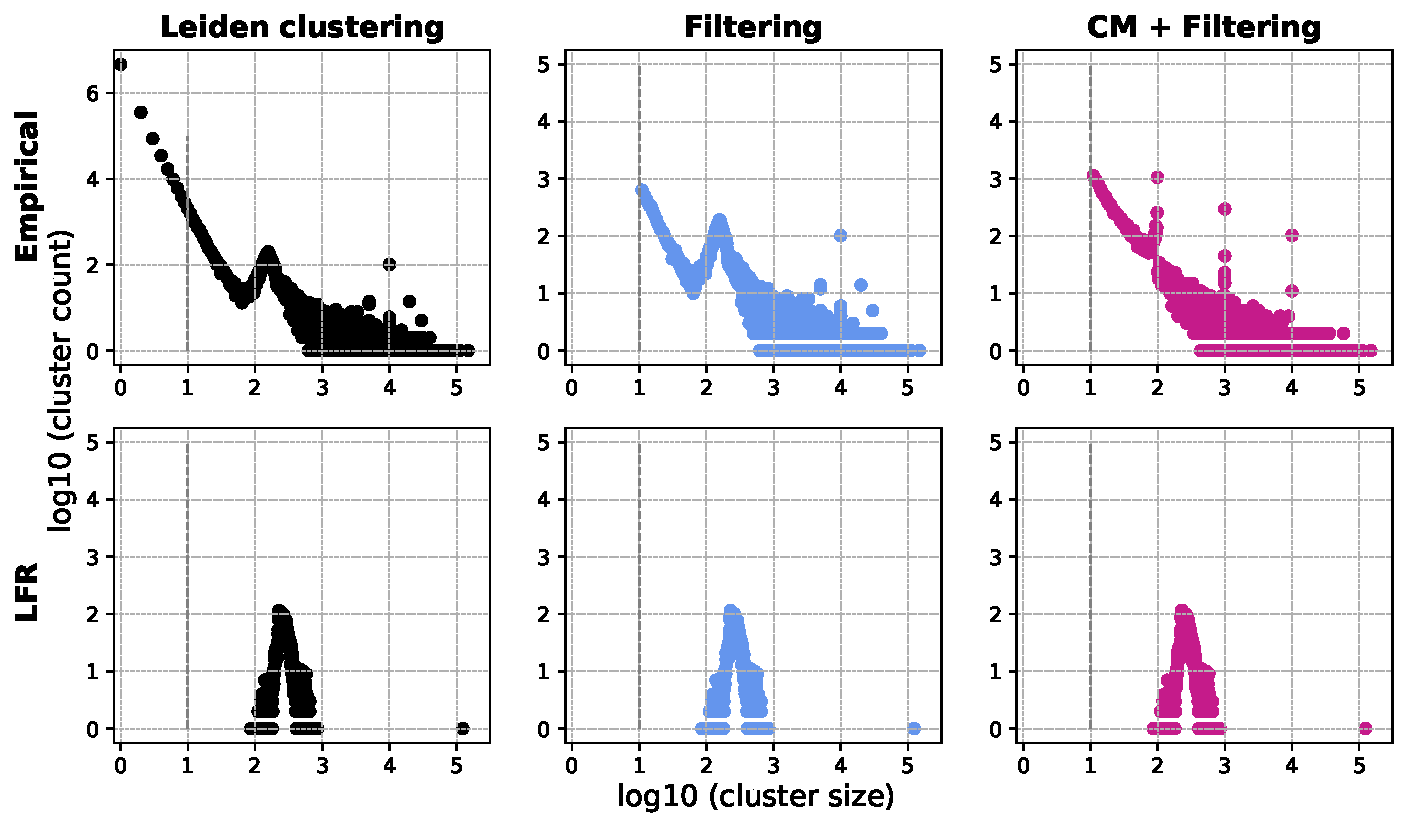
\includegraphics[width=0.62\textwidth]{figs/oc_cm_steps_lfr0001.pdf}
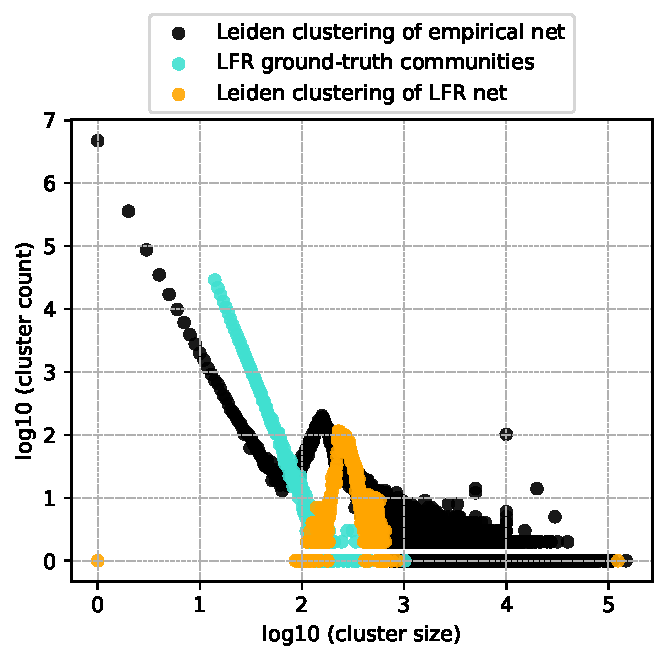
\includegraphics[width=0.37\textwidth]{figs/oc_0001_cm_size.pdf}
\caption[CM pipeline on the empirical Open Citations network and its model LFR graph for r=0.0001]{\textbf{CM pipeline on the empirical Open Citations network and its model LFR graph for r=0.0001.} The left panel shows the community size distribution in each step of running CM and the right panel shows a comparison between the community size distribution of the original Leiden clustering, the LFR ground-truth communities and the Leiden clustering of the LFR network.}
\label{fig:oc-cm-lfr-0001}
\end{figure}

\begin{figure}[h!]
\centering
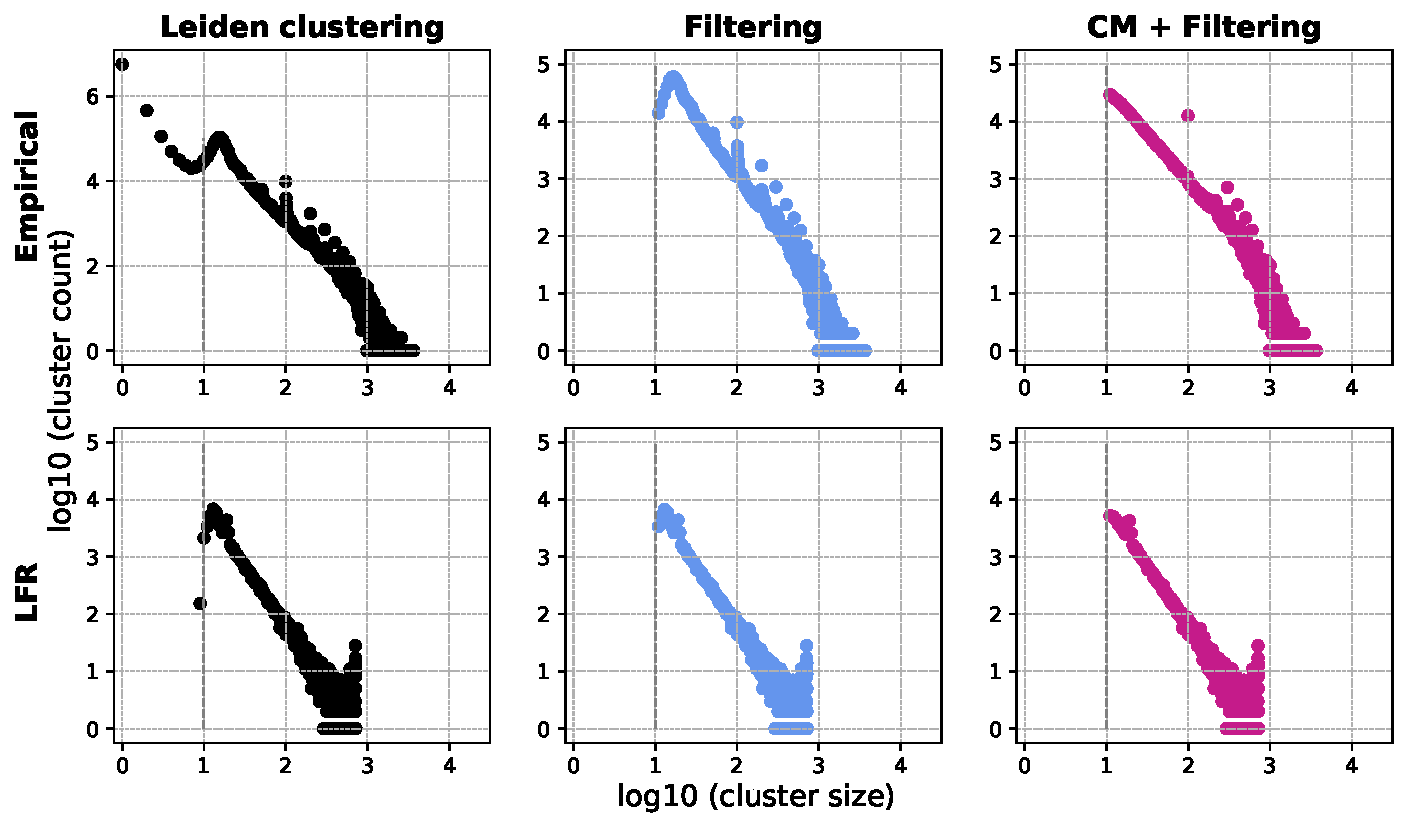
\includegraphics[width=0.62\textwidth]{figs/oc_cm_steps_lfr01.pdf}
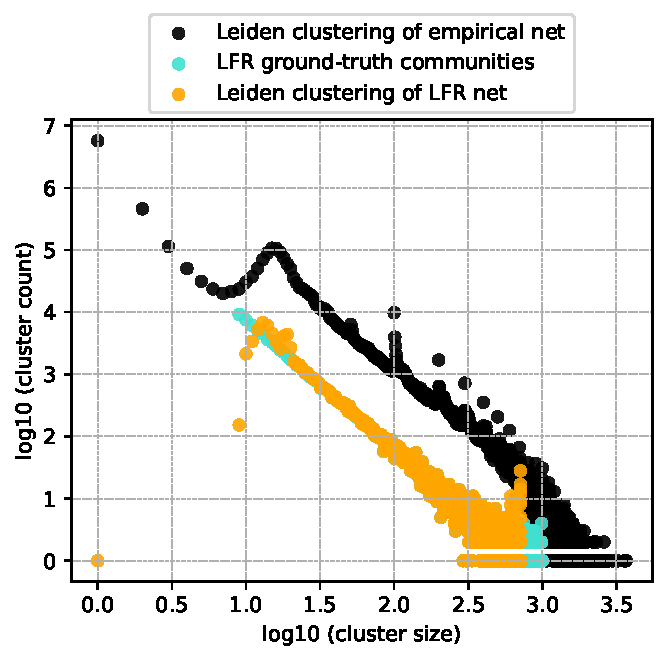
\includegraphics[width=0.37\textwidth]{figs/oc_01_cm_size.pdf}
\caption[CM pipeline on the empirical Open Citations network and its model LFR graph for r=0.01]{\textbf{CM pipeline on the empirical Open Citations network and its model LFR graph for r=0.01.} The left panel shows the community size distribution in each step of running CM and the right panel shows a comparison between the community size distribution of the original Leiden clustering, the LFR ground-truth communities and the Leiden clustering of the LFR network.}
\label{fig:oc-cm-lfr-01}
\end{figure}

\begin{figure}[h!]
\centering
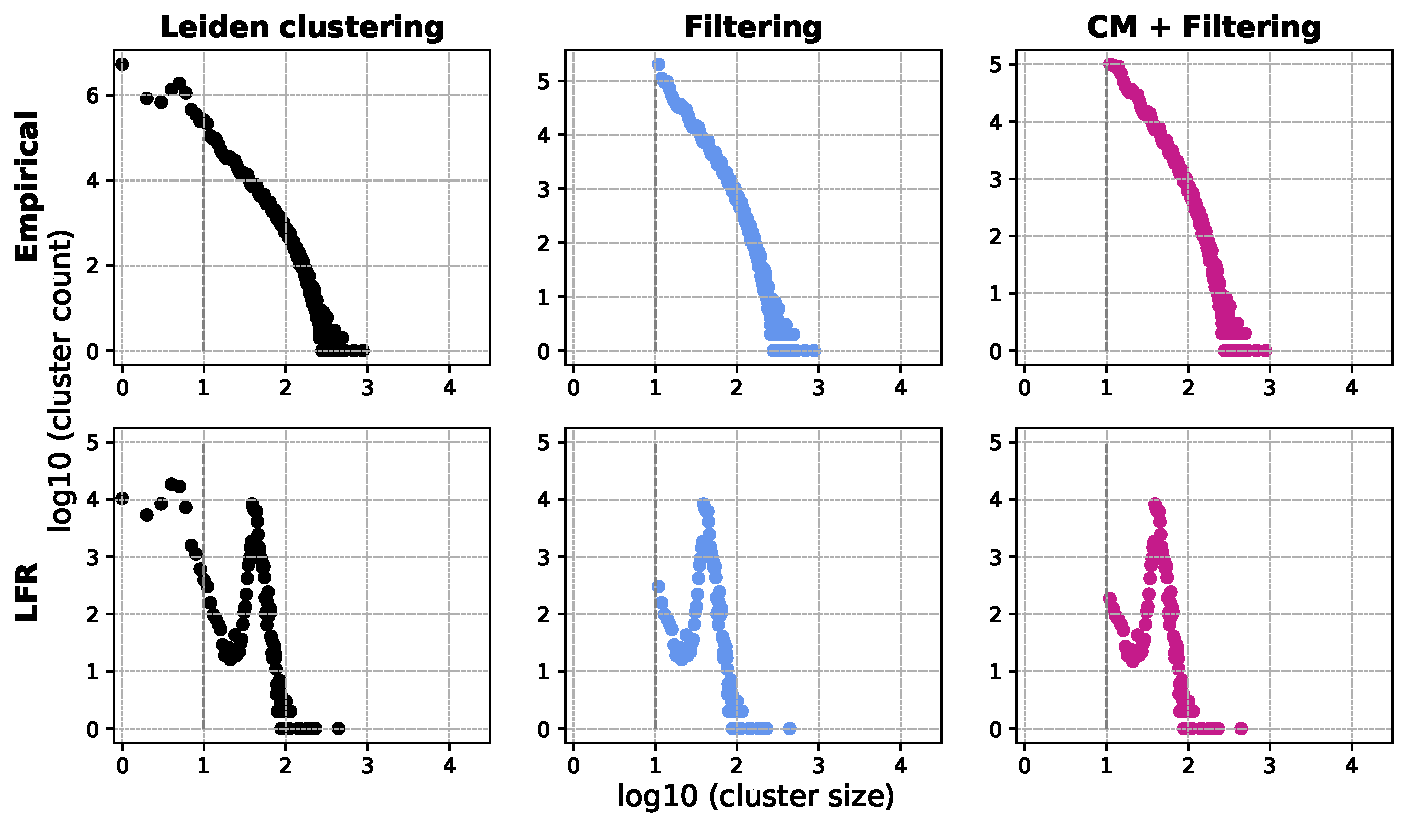
\includegraphics[width=0.62\textwidth]{figs/oc_cm_steps_lfr1.pdf}
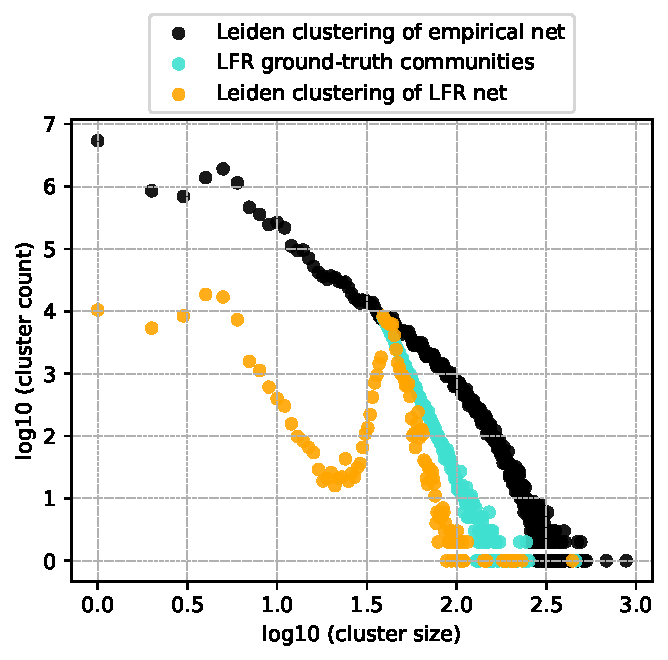
\includegraphics[width=0.37\textwidth]{figs/oc_1_cm_size.pdf}
\caption[CM pipeline on the empirical Open Citations network and its model LFR graph for r=0.1]{\textbf{CM pipeline on the empirical Open Citations network and its model LFR graph for r=0.1.} The left panel shows the community size distribution in each step of running CM and the right panel shows a comparison between the community size distribution of the original Leiden clustering, the LFR ground-truth communities and the Leiden clustering of the LFR network.}
\label{fig:oc-cm-lfr-1}
\end{figure}

\begin{figure}[h!]
\centering
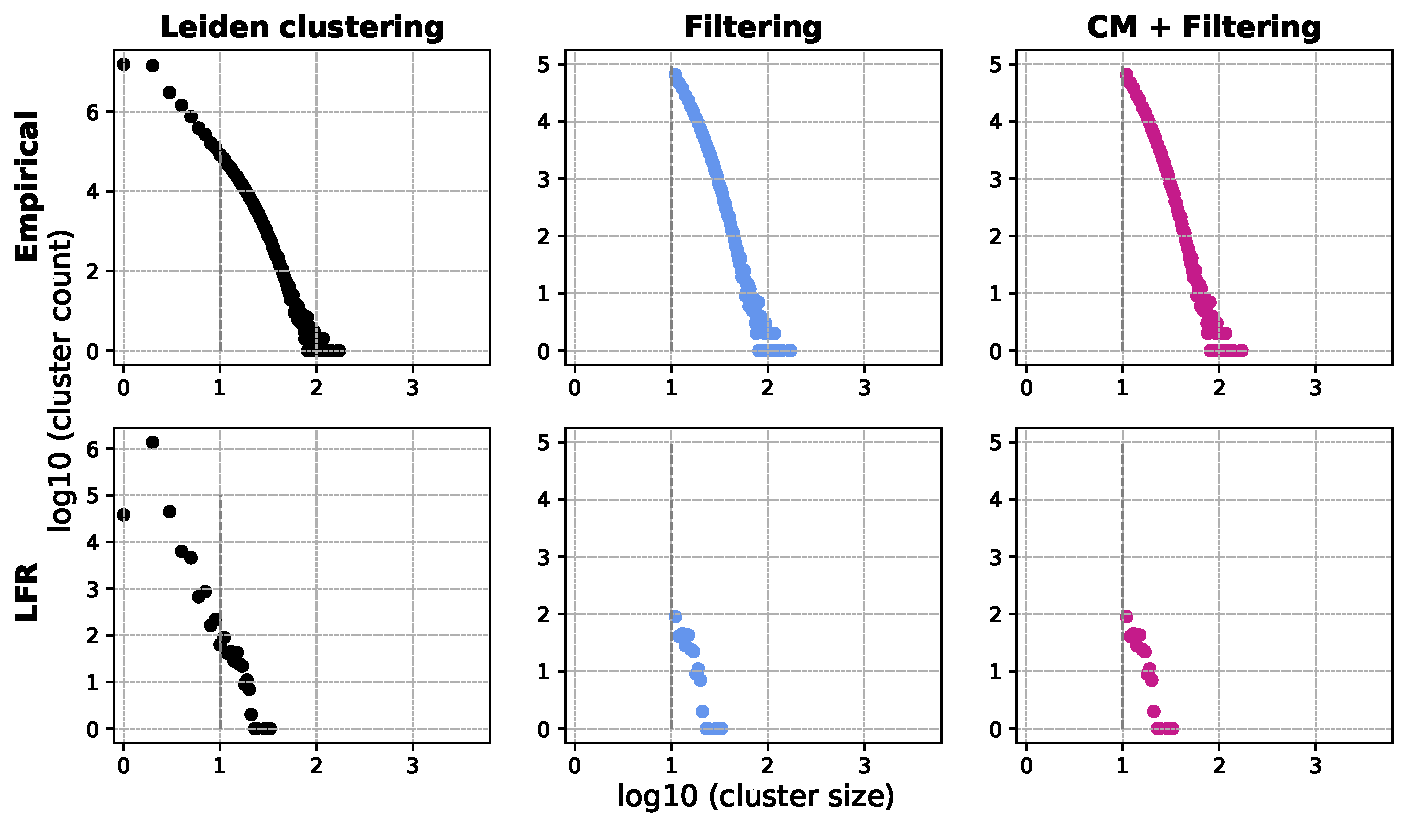
\includegraphics[width=0.62\textwidth]{figs/oc_cm_steps_lfr5.pdf}
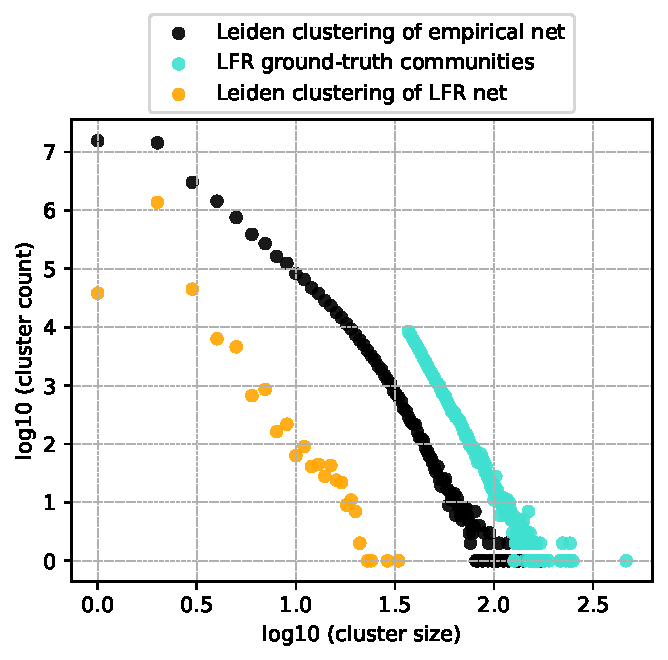
\includegraphics[width=0.37\textwidth]{figs/oc_5_cm_size.pdf}
\caption[CM pipeline on the empirical Open Citations network and its model LFR graph for r=0.5]{\textbf{CM pipeline on the empirical Open Citations network and its model LFR graph for r=0.5.} The left panel shows the community size distribution in each step of running CM and the right panel shows a comparison between the community size distribution of the original Leiden clustering, the LFR ground-truth communities and the Leiden clustering of the LFR network.}
\label{fig:oc-cm-lfr-5}
\end{figure}

\begin{figure}[h!]
\centering
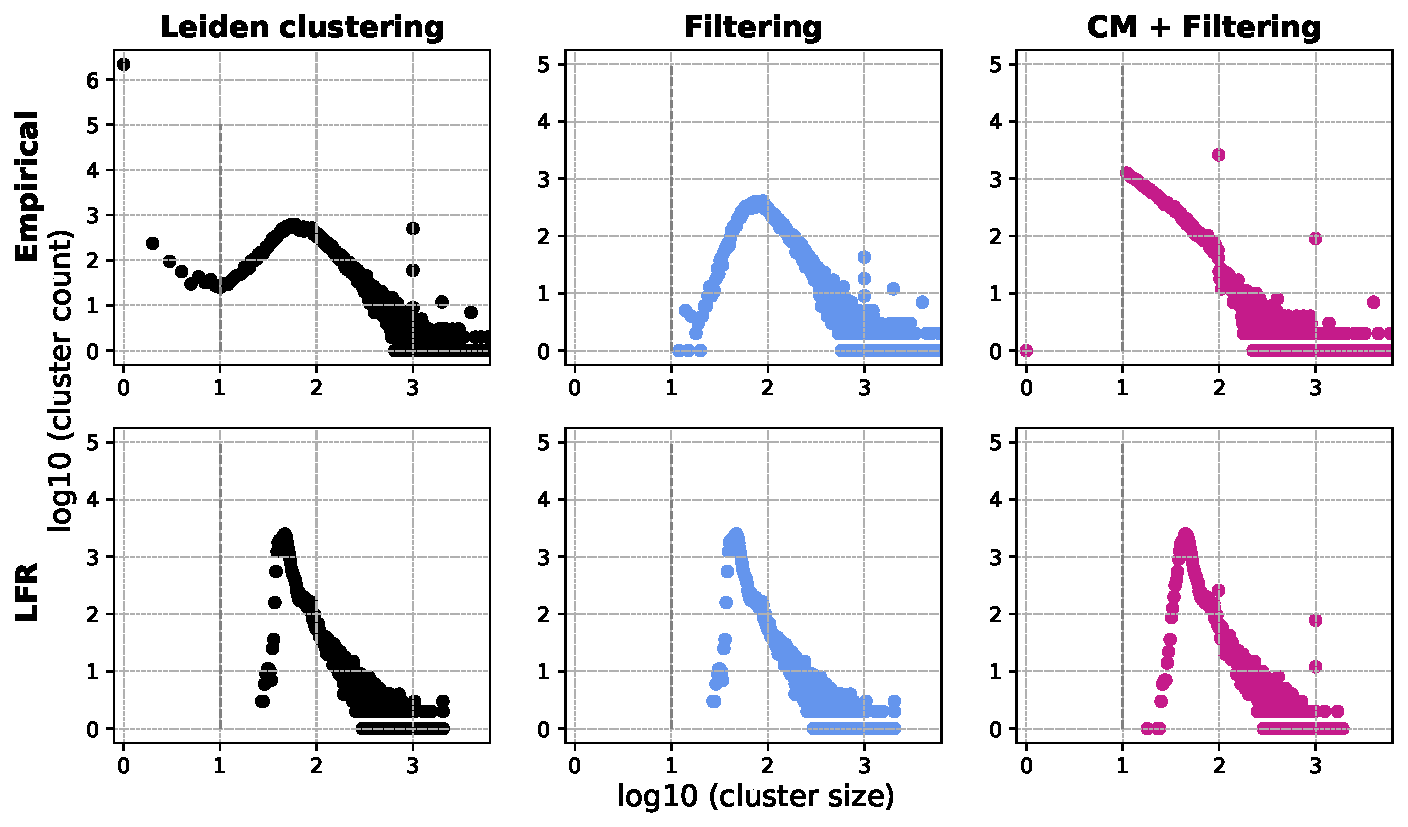
\includegraphics[width=0.62\textwidth]{figs/cen_cm_steps_lfr001.pdf}
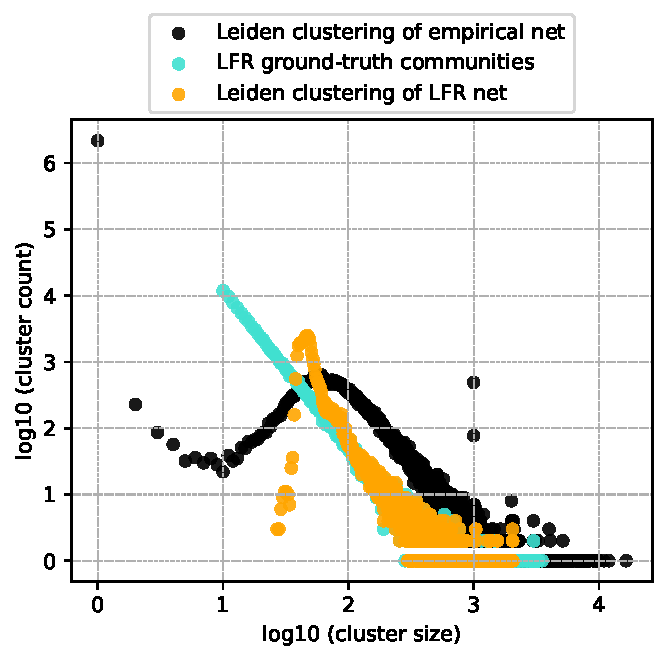
\includegraphics[width=0.37\textwidth]{figs/cen_001_cm_size.pdf}
\caption[CM pipeline on the empirical CEN network and its model LFR graph for r=0.001]{\textbf{CM pipeline on the empirical CEN network and its model LFR graph for r=0.001.} The left panel shows the community size distribution in each step of running CM and the right panel shows a comparison between the community size distribution of the original Leiden clustering, the LFR ground-truth communities and the Leiden clustering of the LFR network.}
\label{fig:cen-cm-lfr-001}
\end{figure}

\begin{figure}[h!]
\centering
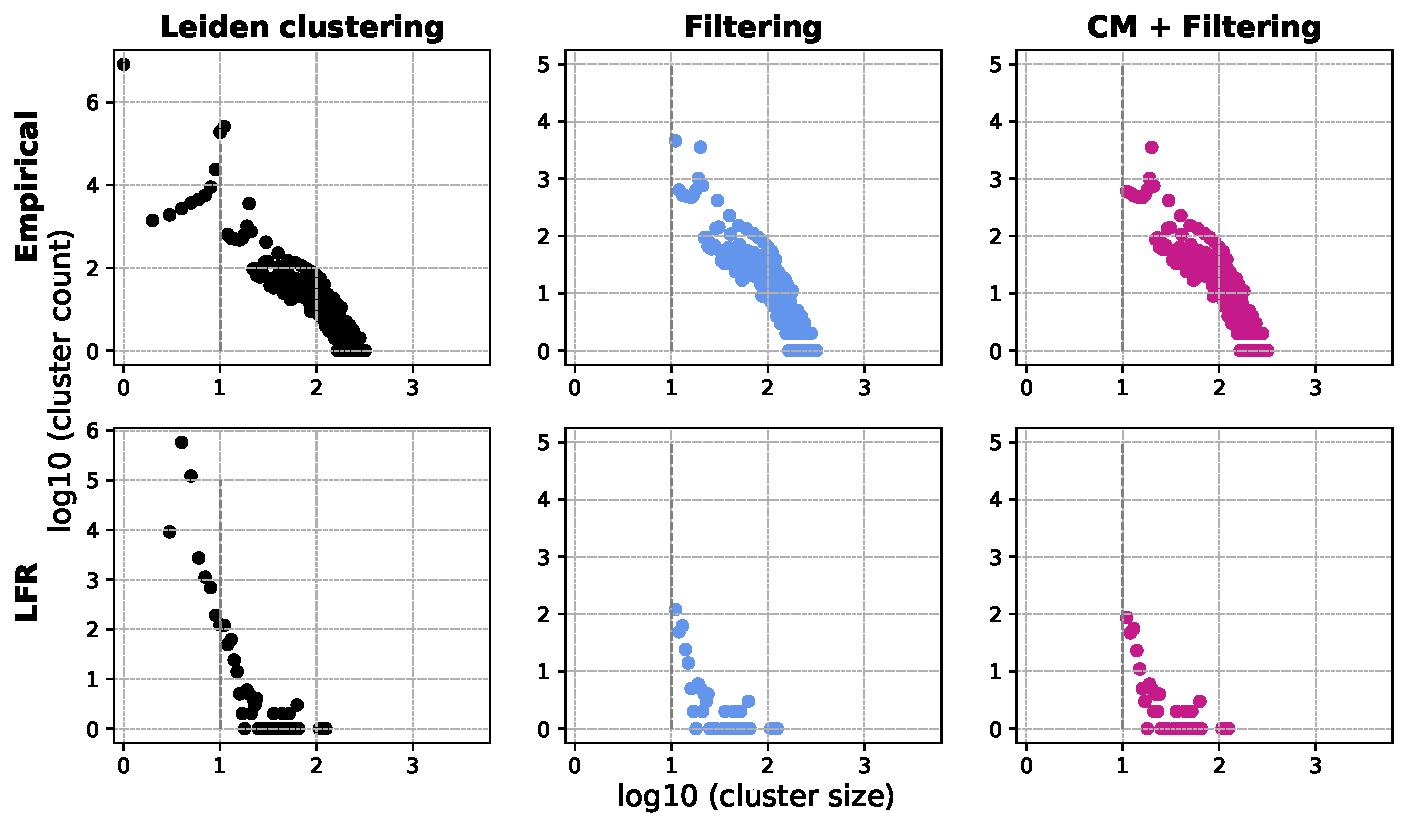
\includegraphics[width=0.62\textwidth]{figs/cen_cm_steps_lfr1.pdf}
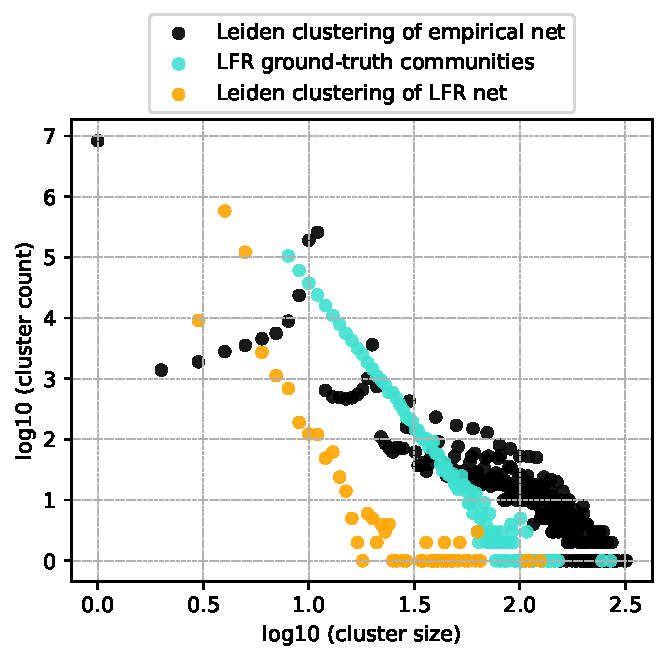
\includegraphics[width=0.37\textwidth]{figs/cen_1_cm_size.pdf}
\caption[CM pipeline on the empirical CEN network and its model LFR graph for r=0.1]{\textbf{CM pipeline on the empirical CEN network and its model LFR graph for r=0.1.} The left panel shows the community size distribution in each step of running CM and the right panel shows a comparison between the community size distribution of the original Leiden clustering, the LFR ground-truth communities and the Leiden clustering of the LFR network.}
\label{fig:cen-cm-lfr-1}
\end{figure}

\begin{figure}[h!]
\centering
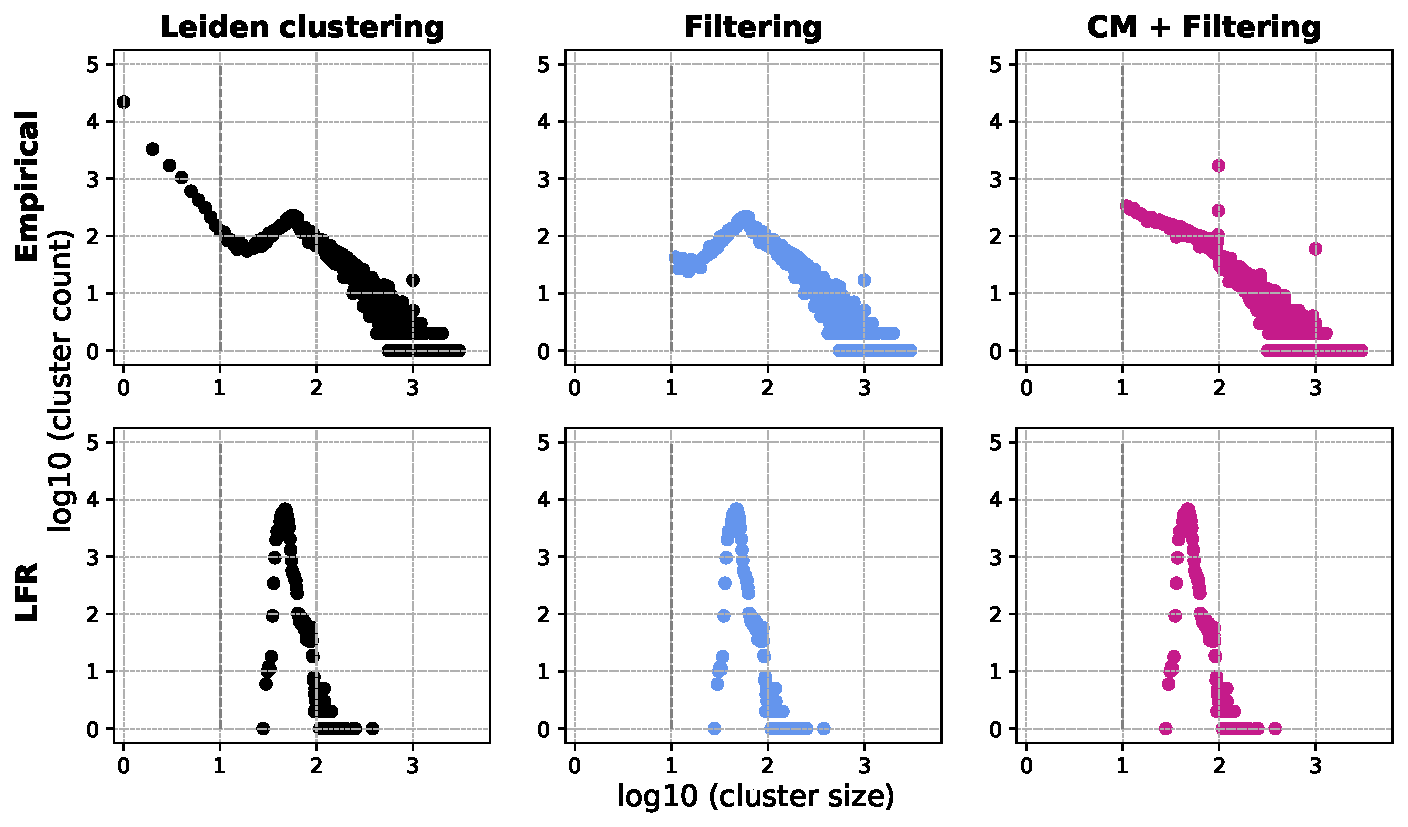
\includegraphics[width=0.62\textwidth]{figs/cit_patents_cm_steps_lfr001.pdf}
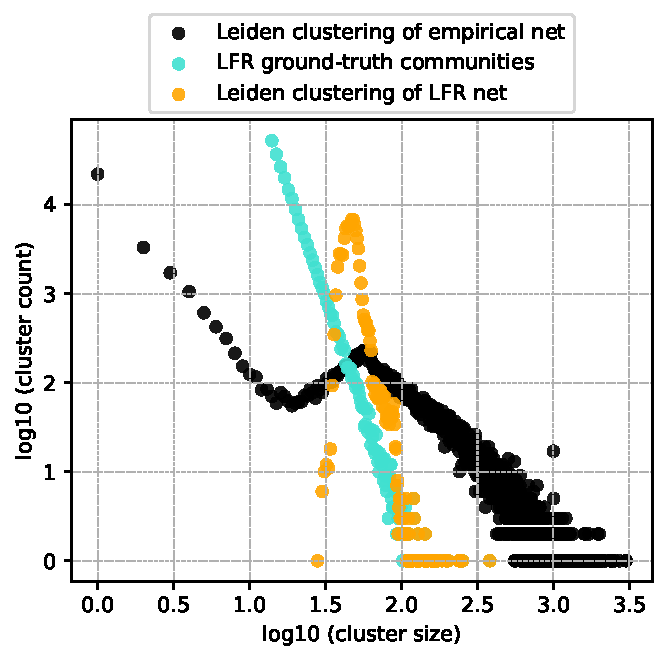
\includegraphics[width=0.37\textwidth]{figs/cit_patents_001_cm_size.pdf}
\caption[CM pipeline on the empirical citation patents network and its model LFR graph for r=0.001]{\textbf{CM pipeline on the empirical citation patents network and its model LFR graph for r=0.001.} The left panel shows the community size distribution in each step of running CM and the right panel shows a comparison between the community size distribution of the original Leiden clustering, the LFR ground-truth communities and the Leiden clustering of the LFR network.}
\label{fig:patents-cm-lfr-001}
\end{figure}


\begin{figure}[h!]
\centering
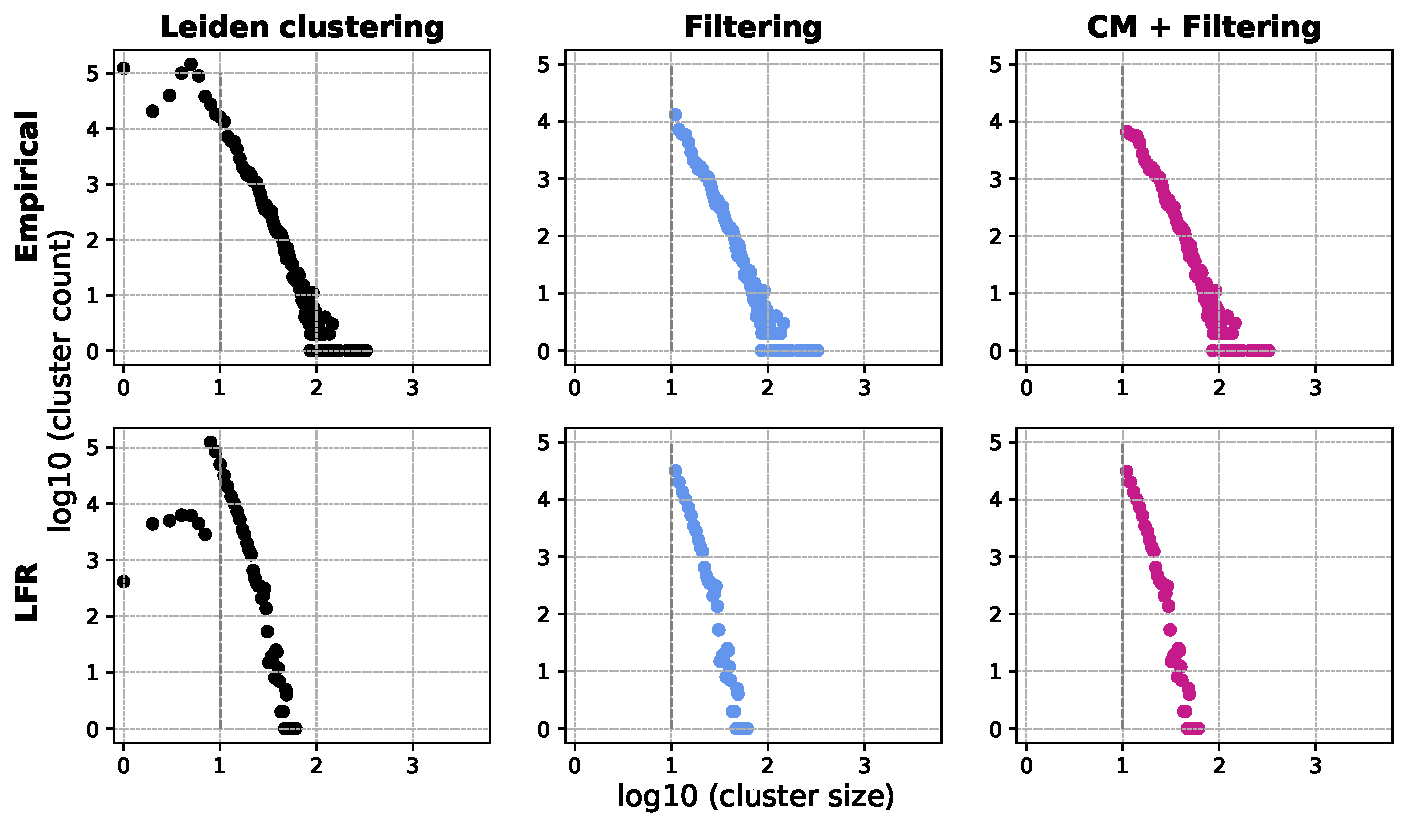
\includegraphics[width=0.62\textwidth]{figs/cit_patents_cm_steps_lfr1.pdf}
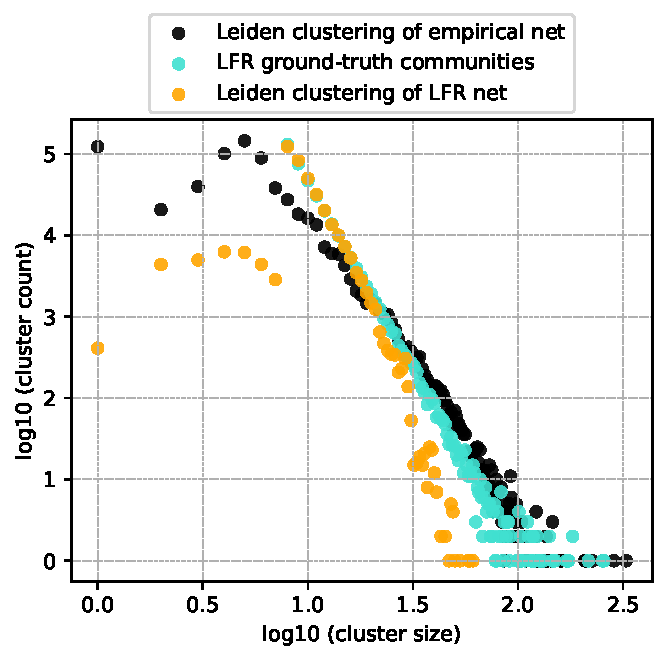
\includegraphics[width=0.37\textwidth]{figs/cit_patents_1_cm_size.pdf}
\caption[CM pipeline on the empirical citation patents network and its model LFR graph for r=0.1]{\textbf{CM pipeline on the empirical citation patents network and its model LFR graph for r=0.1.} The left panel shows the community size distribution in each step of running CM and the right panel shows a comparison between the community size distribution of the original Leiden clustering, the LFR ground-truth communities and the Leiden clustering of the LFR network.}
\label{fig:patents-cm-lfr-1}
\end{figure}

\begin{figure}[h!]
\centering
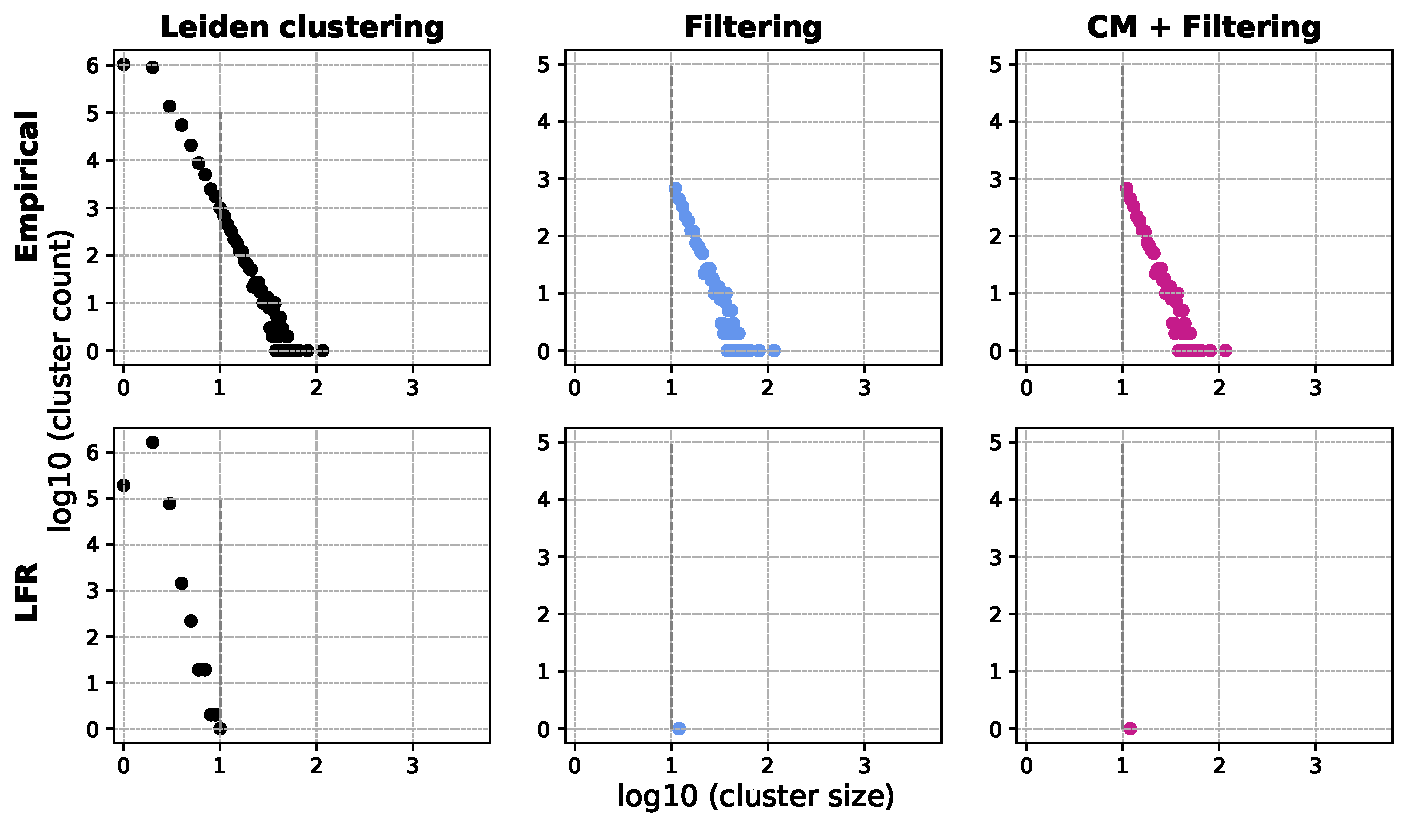
\includegraphics[width=0.62\textwidth]{figs/cit_patents_cm_steps_lfr5.pdf}
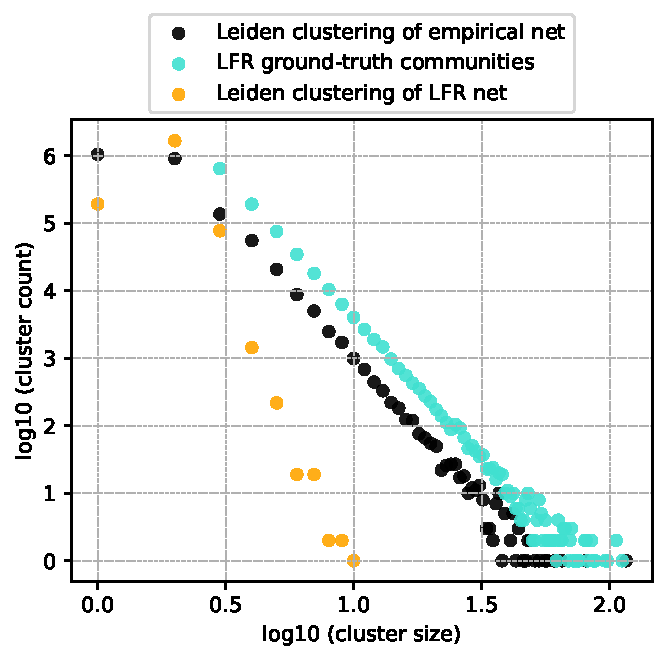
\includegraphics[width=0.37\textwidth]{figs/cit_patents_5_cm_size.pdf}
\caption[CM pipeline on the empirical citation patents network and its model LFR graph for r=0.5]{\textbf{CM pipeline on the empirical citation patents network and its model LFR graph for r=0.5.} The left panel shows the community size distribution in each step of running CM and the right panel shows a comparison between the community size distribution of the original Leiden clustering, the LFR ground-truth communities and the Leiden clustering of the LFR network.}
\label{fig:patents-cm-lfr-5}
\end{figure}

\begin{figure}[h!]
\centering
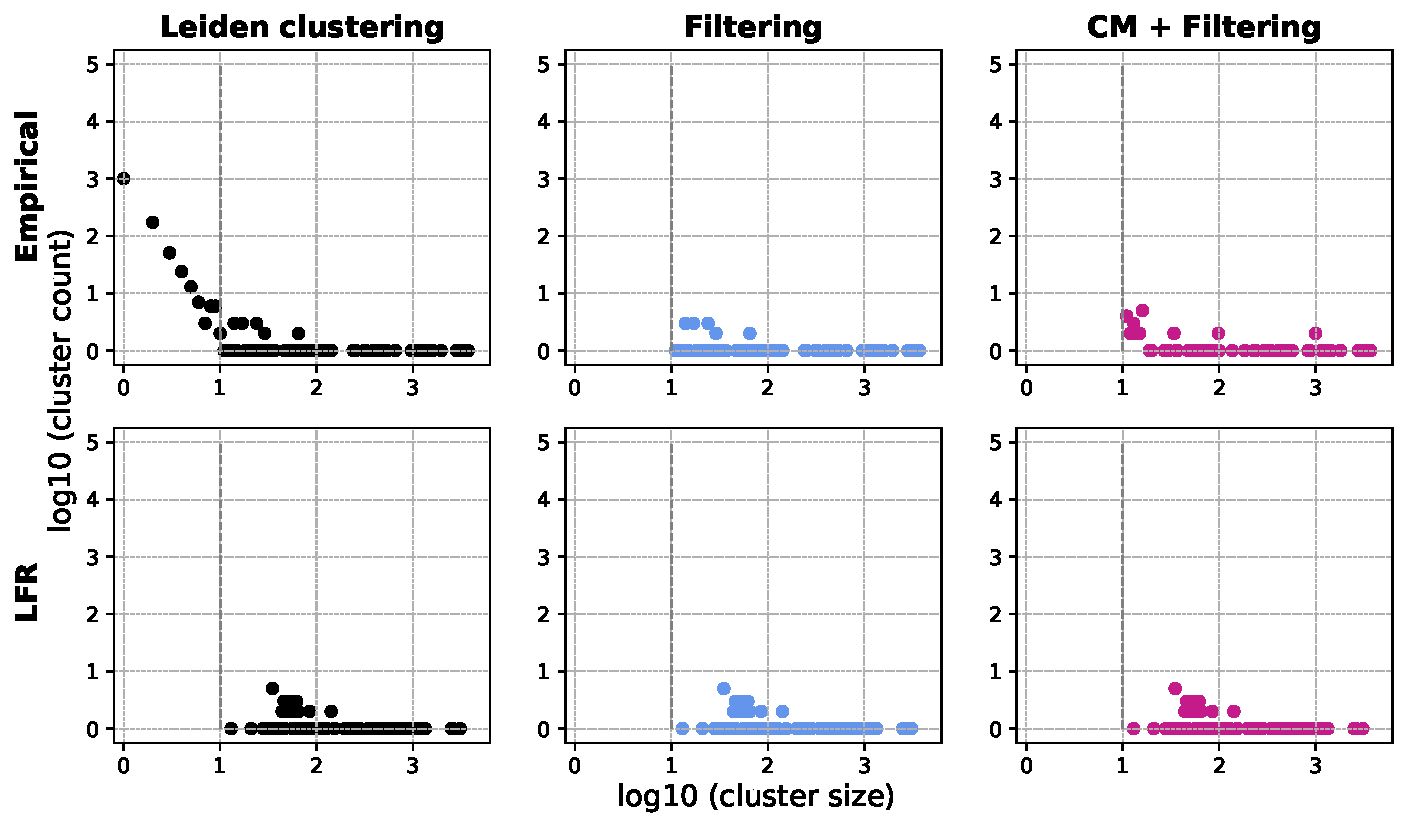
\includegraphics[width=0.62\textwidth]{figs/cit_hepph_cm_steps_lfr001.pdf}
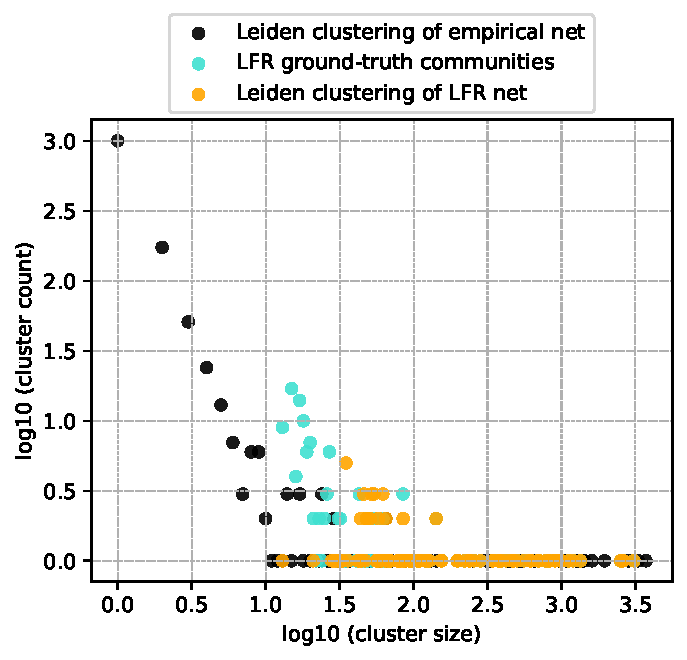
\includegraphics[width=0.37\textwidth]{figs/cit_hepph_001_cm_size.pdf}
\caption[CM pipeline on the empirical physics citation network and its model LFR graph for r=0.001]{\textbf{CM pipeline on the empirical physics citation network and its model LFR graph for r=0.001.} The left panel shows the community size distribution in each step of running CM and the right panel shows a comparison between the community size distribution of the original Leiden clustering, the LFR ground-truth communities and the Leiden clustering of the LFR network.}
\label{fig:hepph-cm-lfr-001}
\end{figure}

\begin{figure}[h!]
\centering
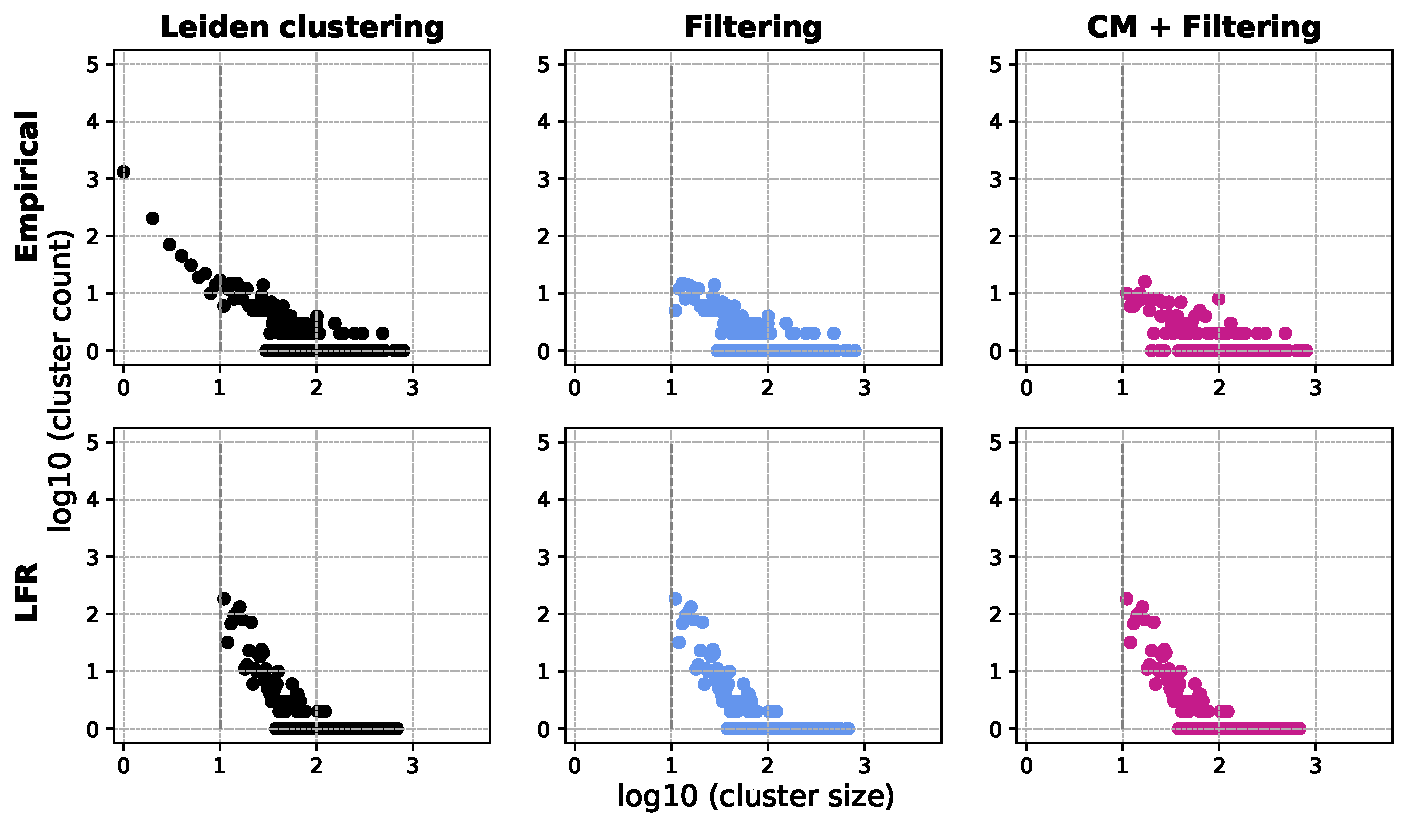
\includegraphics[width=0.62\textwidth]{figs/cit_hepph_cm_steps_lfr01.pdf}
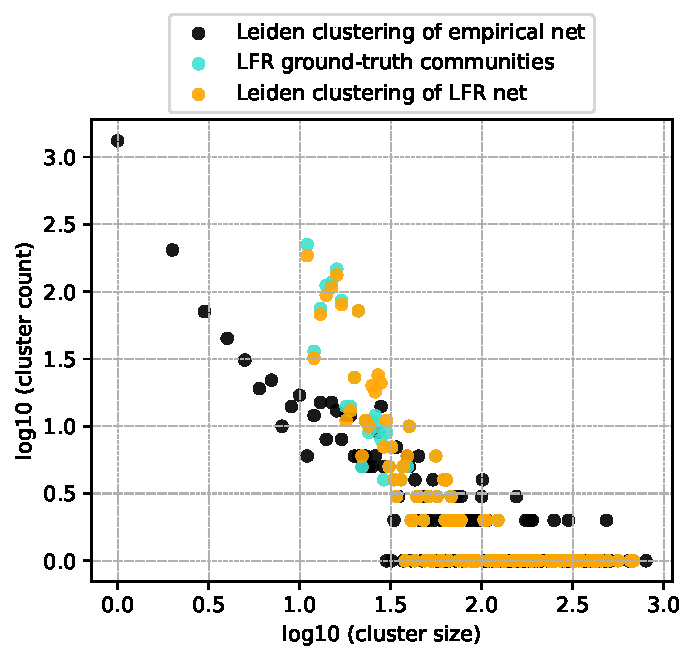
\includegraphics[width=0.37\textwidth]{figs/cit_hepph_01_cm_size.pdf}
\caption[CM pipeline on the empirical High Energy Physics Citation network and its model LFR graph for r=0.01]{\textbf{CM pipeline on the empirical physics citation network and its model LFR graph for r=0.01.} The left panel shows the community size distribution in each step of running CM and the right panel shows a comparison between the community size distribution of the original Leiden clustering, the LFR ground-truth communities and the Leiden clustering of the LFR network.}
\label{fig:hepph-cm-lfr-01}
\end{figure}

\begin{figure}[h!]
\centering
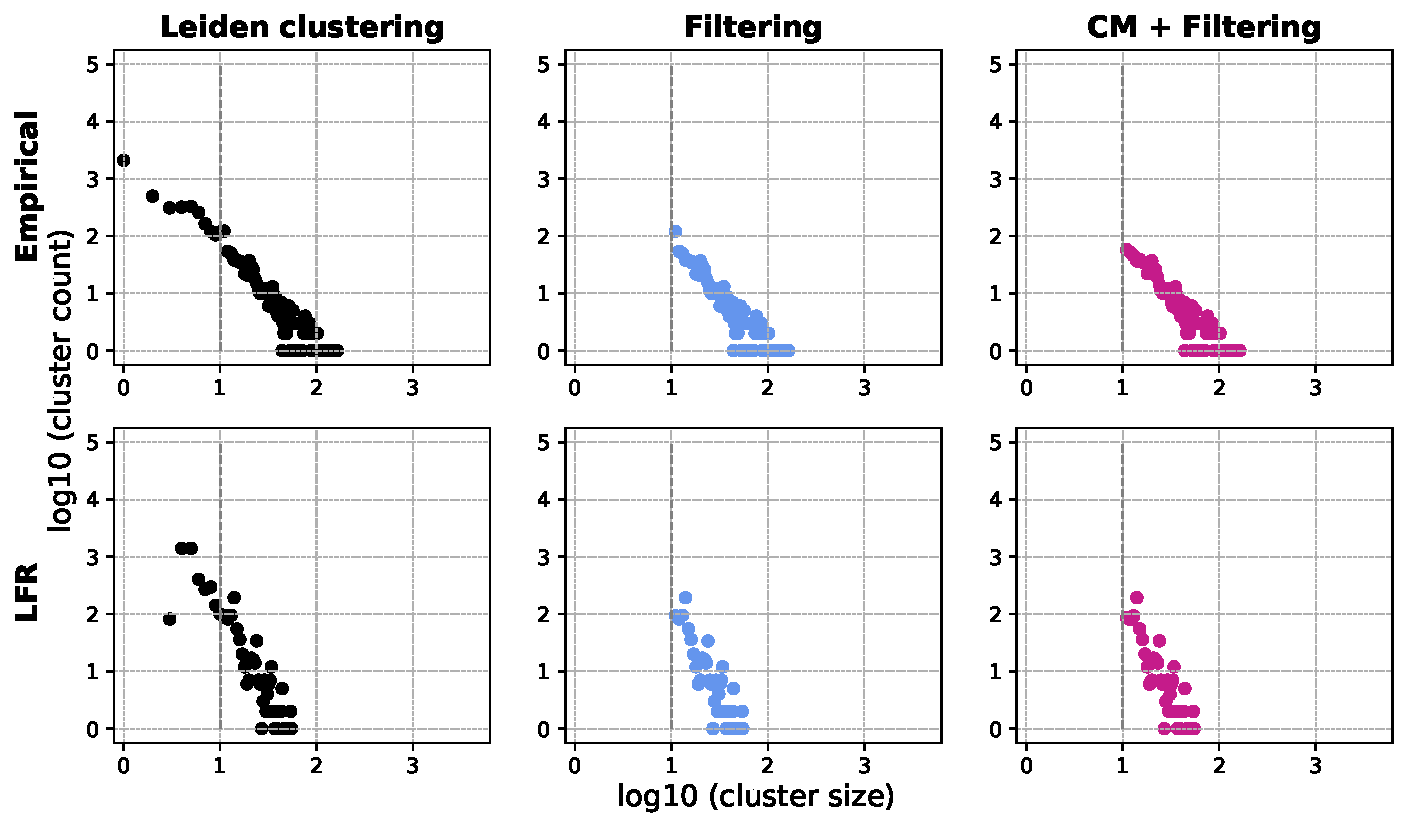
\includegraphics[width=0.62\textwidth]{figs/cit_hepph_cm_steps_lfr1.pdf}
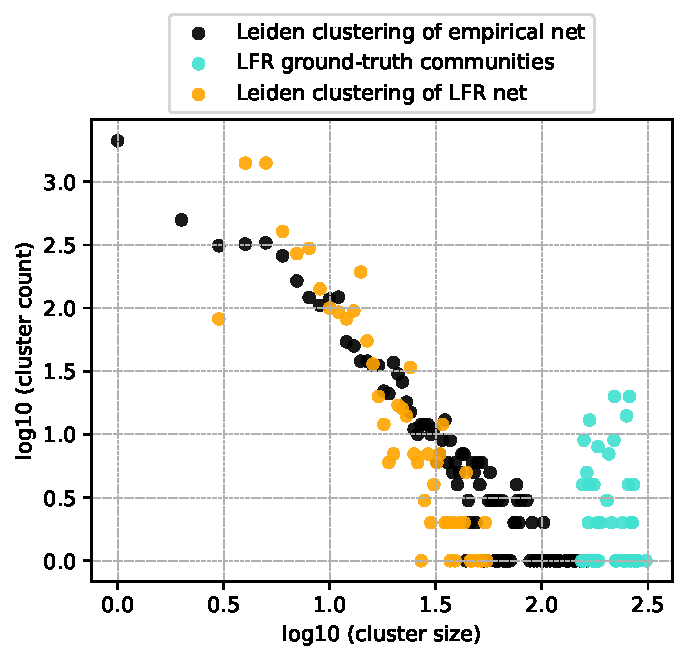
\includegraphics[width=0.37\textwidth]{figs/cit_hepph_1_cm_size.pdf}
\caption[CM pipeline on the empirical physics citation network and its model LFR graph for r=0.1]{\textbf{CM pipeline on the empirical physics citation network and its model LFR graph for r=0.1.} The left panel shows the community size distribution in each step of running CM and the right panel shows a comparison between the community size distribution of the original Leiden clustering, the LFR ground-truth communities and the Leiden clustering of the LFR network.}
\label{fig:hepph-cm-lfr-1}
\end{figure}

\begin{figure}[h!]
\centering
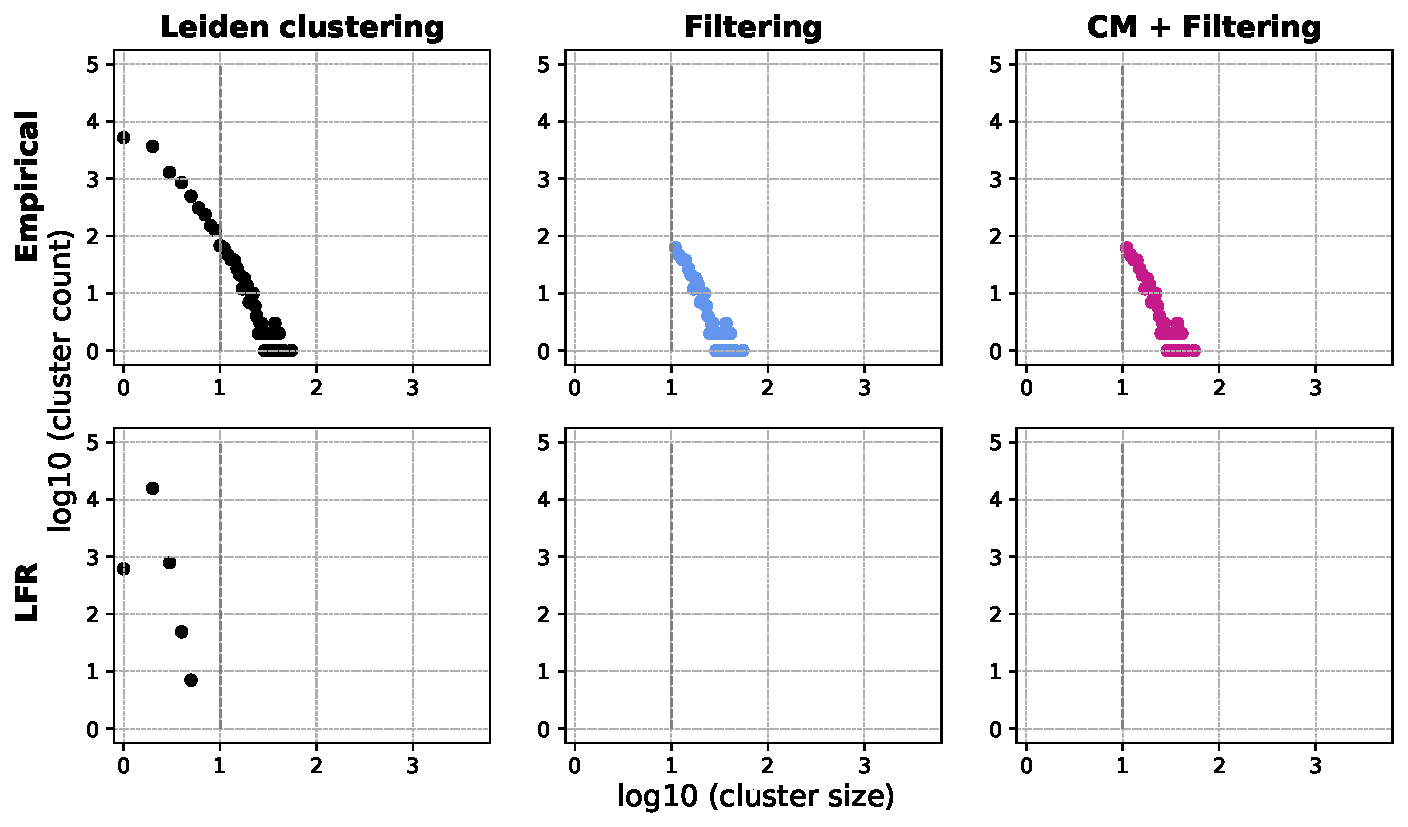
\includegraphics[width=0.62\textwidth]{figs/cit_hepph_cm_steps_lfr5.pdf}
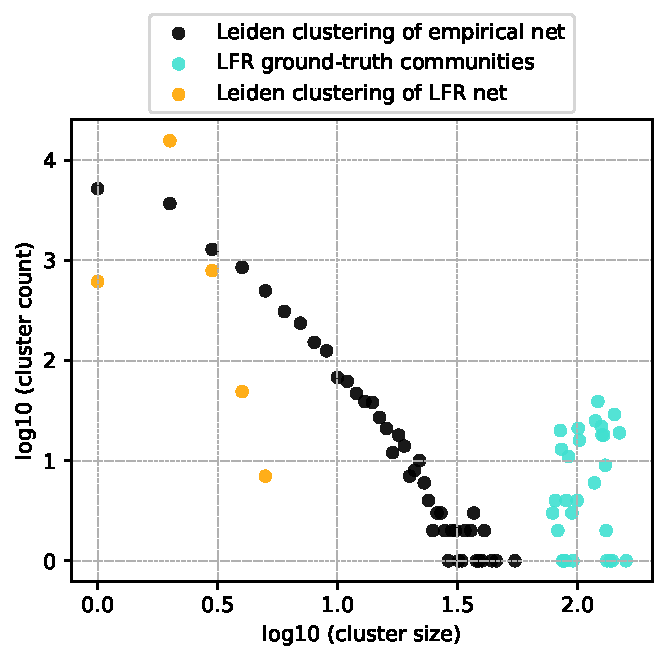
\includegraphics[width=0.37\textwidth]{figs/cit_hepph_5_cm_size.pdf}
\caption[CM pipeline on the empirical physics citation network and its model LFR graph for r=0.5]{\textbf{CM pipeline on the empirical physics citation network and its model LFR graph for r=0.5.} The left panel shows the community size distribution in each step of running CM and the right panel shows a comparison between the community size distribution of the original Leiden clustering, the LFR ground-truth communities and the Leiden clustering of the LFR network.}
\label{fig:hepph-cm-lfr-5}
\end{figure}

\begin{figure}[h!]
\centering
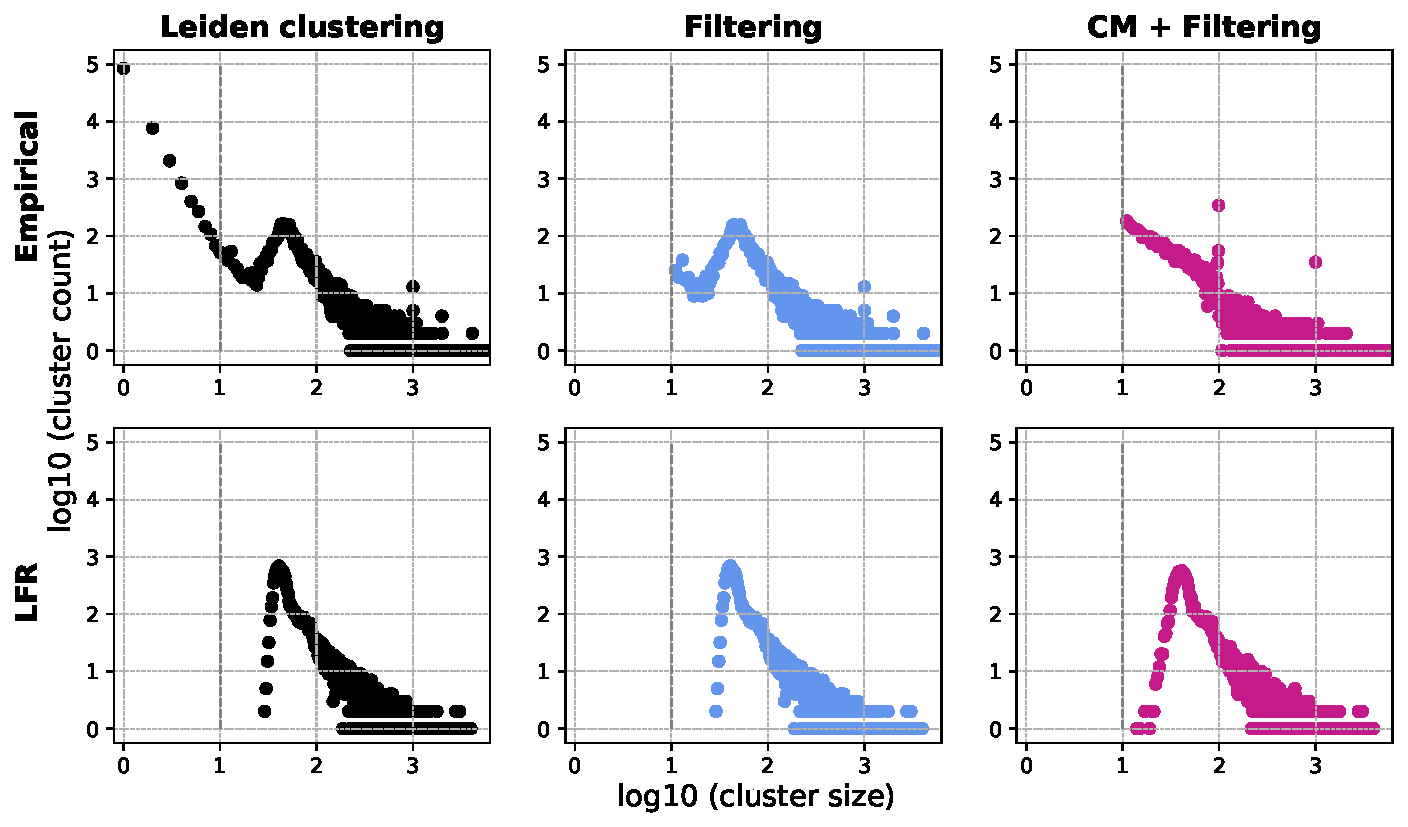
\includegraphics[width=0.62\textwidth]{figs/wiki_topcats_cm_steps_lfr001.pdf}
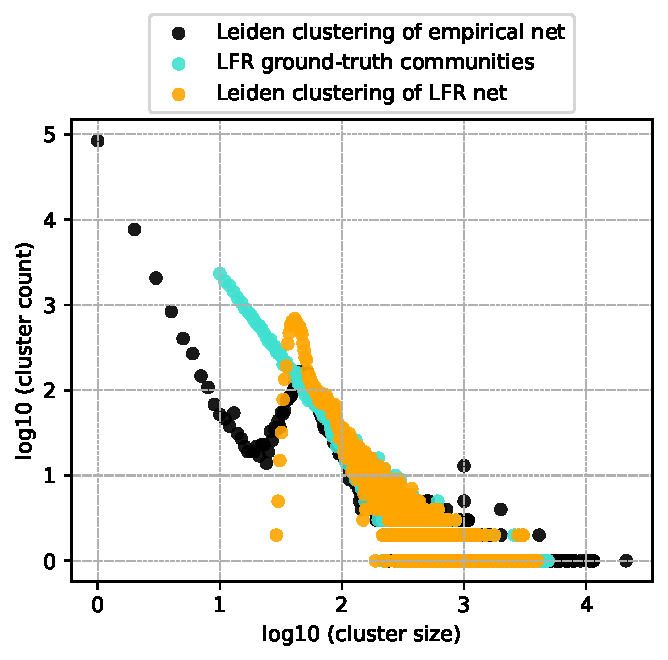
\includegraphics[width=0.37\textwidth]{figs/wiki_topcats_001_cm_size.pdf}
\caption[CM pipeline on the Wikipedia hyperlinks network and its model LFR graph for r=0.001]{\textbf{CM pipeline on the empirical Wikipedia hyperlinks network and its model LFR graph for r=0.001.} The left panel shows the community size distribution in each step of running CM and the right panel shows a comparison between the community size distribution of the original Leiden clustering, the LFR ground-truth communities and the Leiden clustering of the LFR network.}
\label{fig:wikitopcats-cm-lfr-001}
\end{figure}

\begin{figure}[h!]
\centering
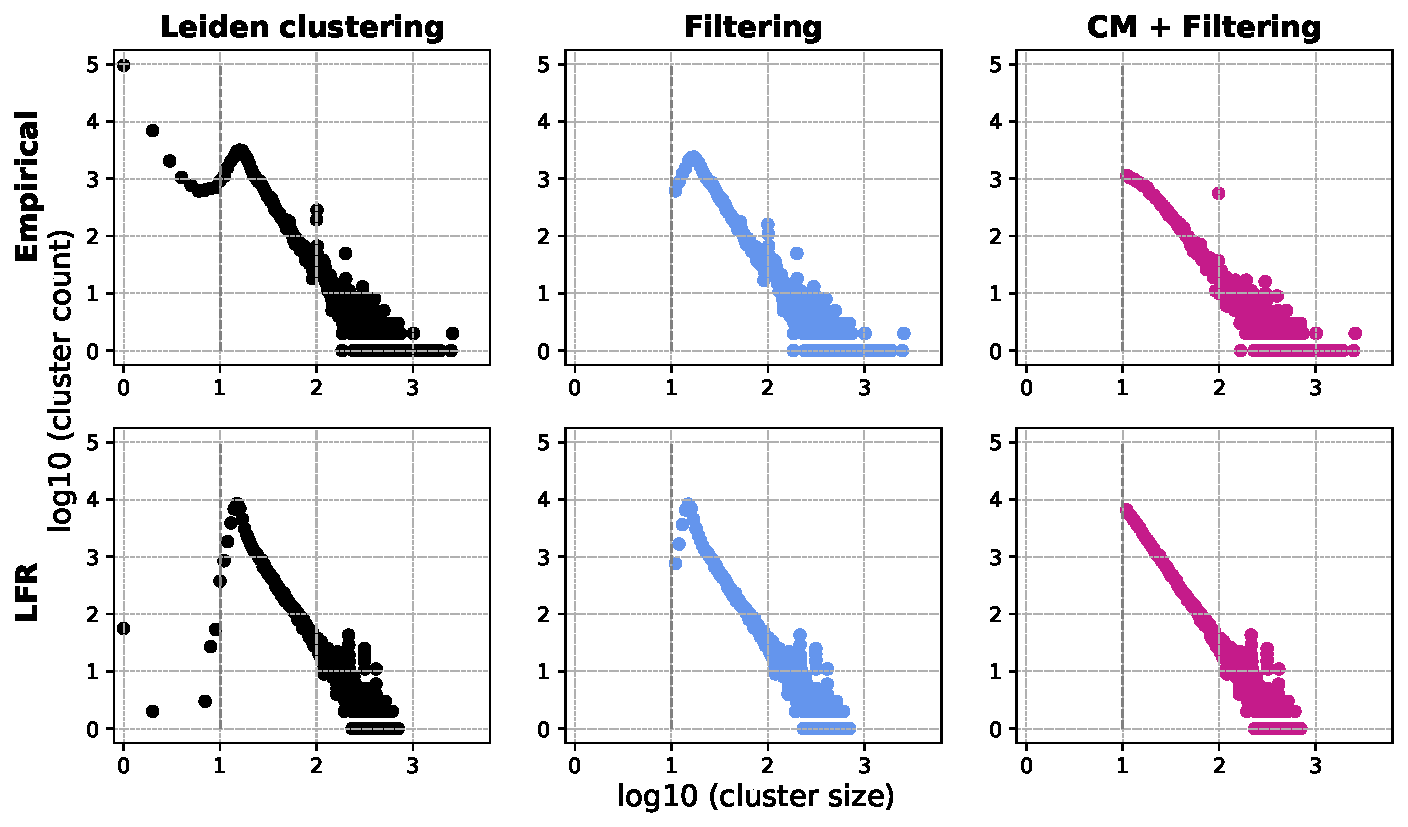
\includegraphics[width=0.62\textwidth]{figs/wiki_topcats_cm_steps_lfr01.pdf}
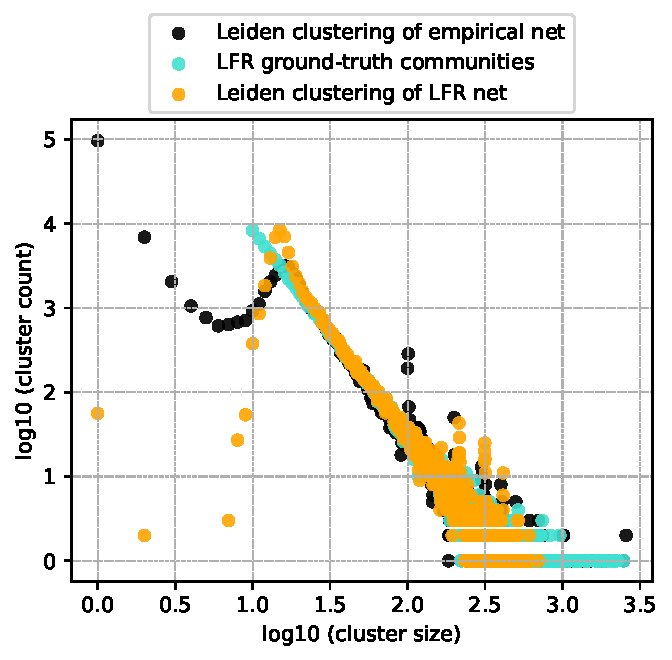
\includegraphics[width=0.37\textwidth]{figs/wiki_topcats_01_cm_size.pdf}
\caption[CM pipeline on the Wikipedia hyperlinks network and its model LFR graph for r=0.01]{\textbf{CM pipeline on the empirical Wikipedia hyperlinks network and its model LFR graph for r=0.01.} The left panel shows the community size distribution in each step of running CM and the right panel shows a comparison between the community size distribution of the original Leiden clustering, the LFR ground-truth communities and the Leiden clustering of the LFR network.}
\label{fig:wikitopcats-cm-lfr-01}
\end{figure}

\begin{figure}[h!]
\centering
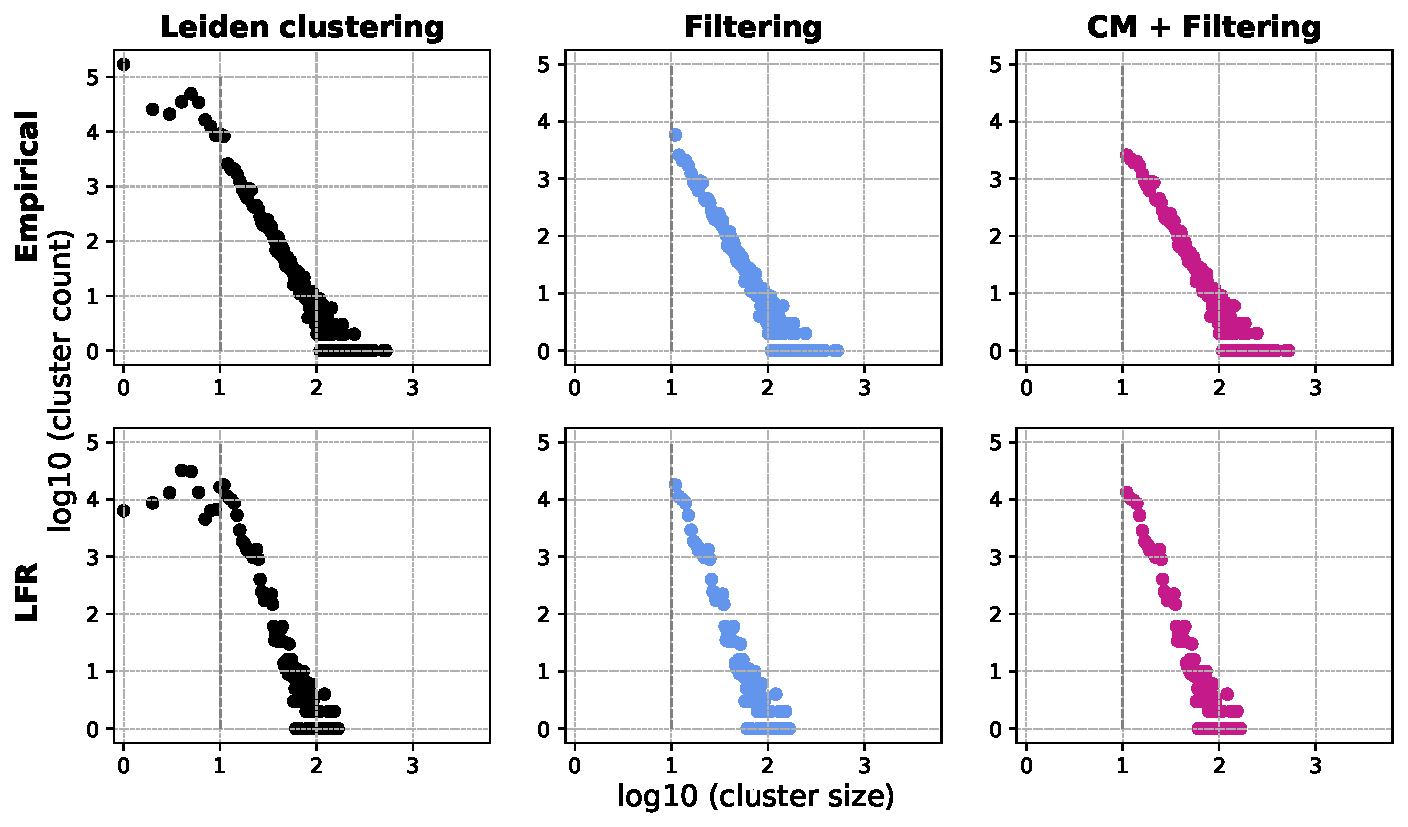
\includegraphics[width=0.62\textwidth]{figs/wiki_topcats_cm_steps_lfr1.pdf}
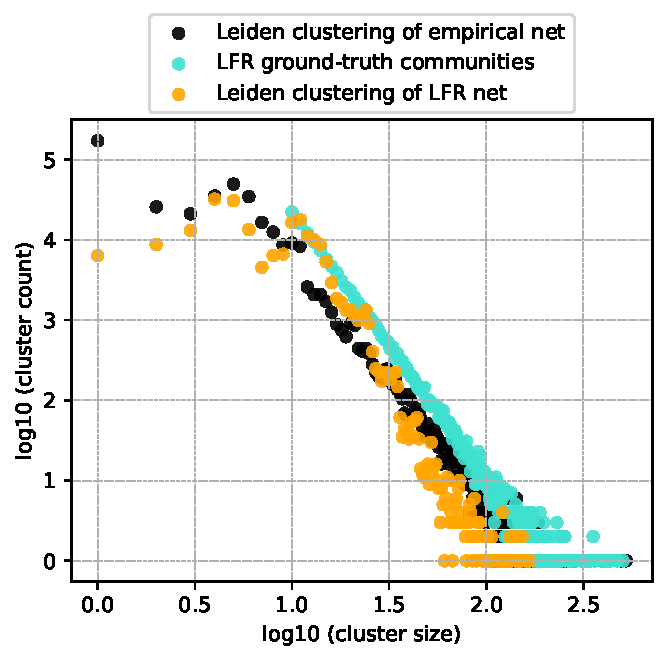
\includegraphics[width=0.37\textwidth]{figs/wiki_topcats_1_cm_size.pdf}
\caption[CM pipeline on the Wikipedia hyperlinks network and its model LFR graph for r=0.1]{\textbf{CM pipeline on the empirical Wikipedia hyperlinks network and its model LFR graph for r=0.1.} The left panel shows the community size distribution in each step of running CM and the right panel shows a comparison between the community size distribution of the original Leiden clustering, the LFR ground-truth communities and the Leiden clustering of the LFR network.}
\label{fig:wikitopcats-cm-lfr-1}
\end{figure}

\begin{figure}[h!]
\centering
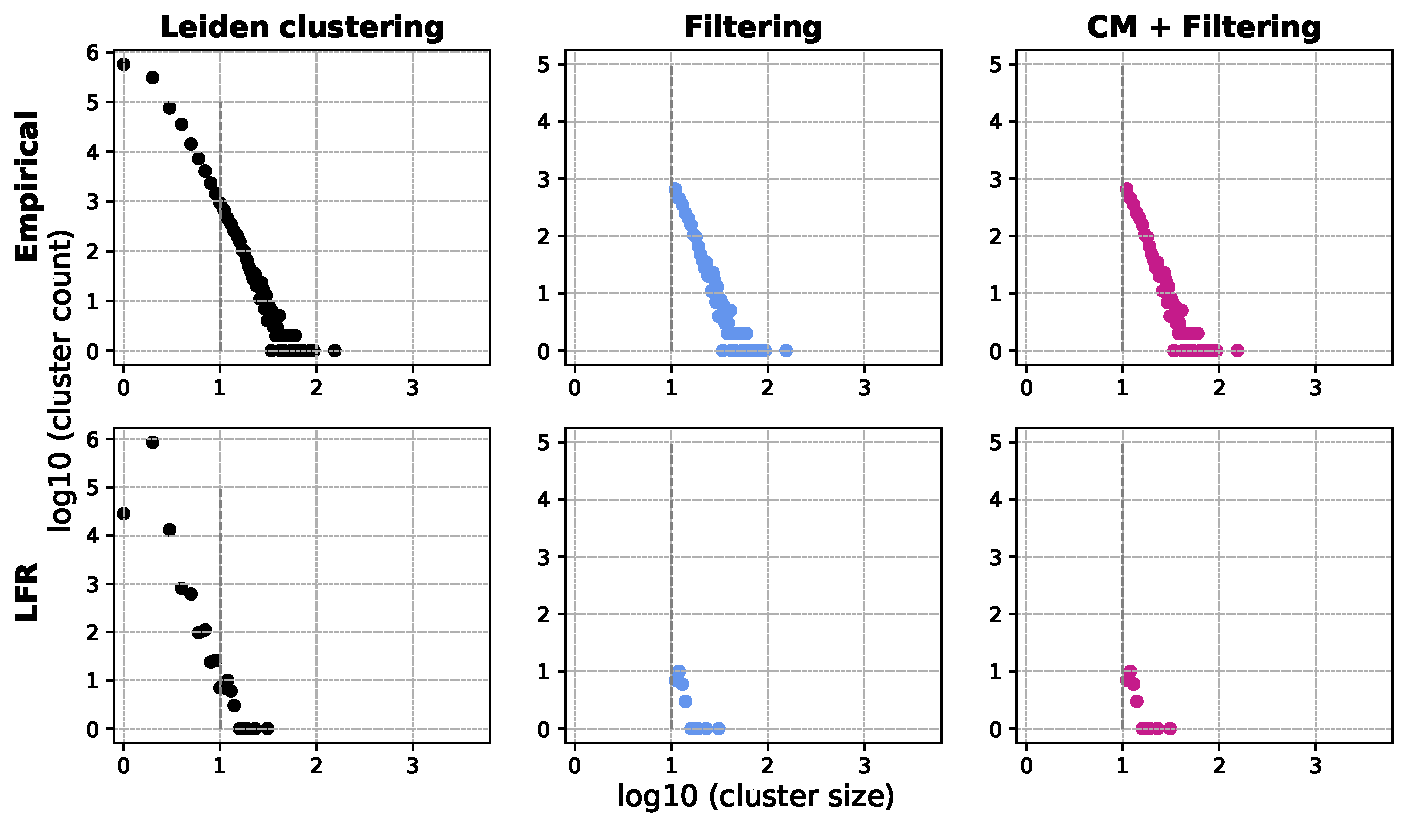
\includegraphics[width=0.62\textwidth]{figs/wiki_topcats_cm_steps_lfr5.pdf}
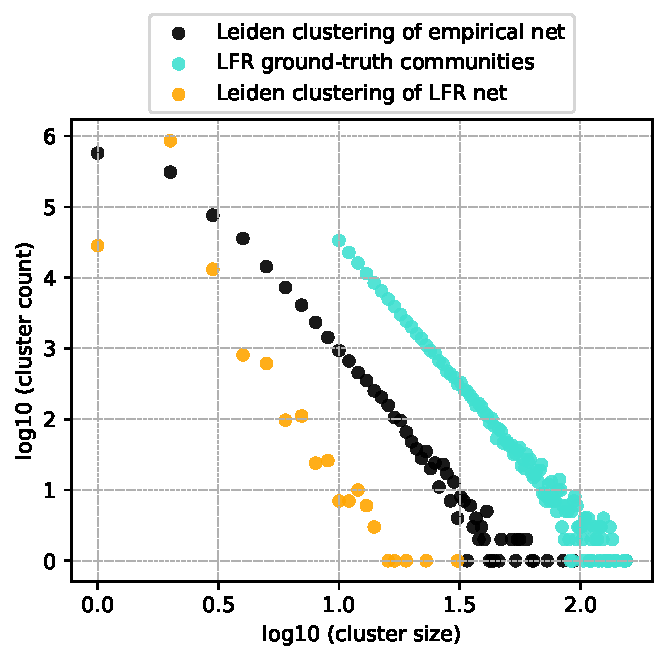
\includegraphics[width=0.37\textwidth]{figs/wiki_topcats_5_cm_size.pdf}
\caption[CM pipeline on the Wikipedia hyperlinks network and its model LFR graph for r=0.5]{\textbf{CM pipeline on the empirical Wikipedia hyperlinks network and its model LFR graph for r=0.5.} The left panel shows the community size distribution in each step of running CM and the right panel shows a comparison between the community size distribution of the original Leiden clustering, the LFR ground-truth communities and the Leiden clustering of the LFR network.}
\label{fig:wikitopcats-cm-lfr-5}
\end{figure}

\clearpage

\begin{table}[ht]
\centering
\begin{tabular}{rrrrrr}
  \hline
  k value & clus count & node cov & min & med & max       \\ \hline
  10      & 2569       & 23.6     & 11  & 40  & 6,650,349 \\
  \hline
\end{tabular}
\caption[IKC clusters of size at least 11 for the Open Citations Network]{\textbf{IKC clusters of size at least 11 for the Open Citations Network} The Open Citations Network (Materials and Methods) consisting of 75,025,194 nodes and 1,363,605,603 edges was clustered with the IKC algorithm using a k value of 10.
Node coverage is the percentage of nodes in the network found in clusters of size at least 11. Minimum, median, and max cluster sizes, restricted to clusters of size at least 11, are shown in the last three columns. }
\label{tab:IKC-11-OC-basicstats}
\end{table}

\begin{table}[ht]
\centering
\begin{tabular}{lrrrrrr}
  \hline
  clustering & k\_value & clus\_count & node\_cov & min & med & max \\ \hline
  IKC        & 10       & 3999        & 19.5      & 11  & 45  & 6,650,087 \\
  \hline
\end{tabular}
\caption[Identifying well connected clusters from IKC clustering of the OC]{\textbf{Identifying well connected clusters from IKC clustering of the OC} Following the same procedure as Leiden, the clusters were limited to those of size 11 or greater, then depleted of trees, then processed by CM, and then filtered to remove any clusters of size 10 or less as well as trees. However, this result excludes three large (size 100,000+) clusters of IKC for which CM could not run. In order to make CM scalable to the OpenCitations network, we processed all clusters above size 100,000 individually through CM and processed all clusters size 100,000 or below as one clustering through CM. There were 19 clusters that were greater than size 100,000, of which 3 clusters failed to run through CM. The CM results of the 16 clusters were combined with the CM result of the clusters size 100,000 or below to produce the final clustering whose cluster statistics are reported in the table.}
\label{tab:CM-IKC-11-OC-basicstats}
\end{table}

\begin{table}[ht]
\centering
\begin{tabular}{rrrrrr}
  \hline
  k value & clus count & node cov & min & med & max       \\ \hline
  10       & 128         & 3.8       & 14  & 79  & 214,877 \\
  \hline
\end{tabular}
\caption[IKC clusters of size at least 11 for the CEN]{\textbf{IKC clusters of size at least 11 for the CEN} The Curated Exososome Network was clustered with the IKC algorithm using a k value of 10.
Node coverage is the percentage of nodes in the network found in clusters of size at least 11. Minimum, median, and max cluster sizes, restricted to clusters of size at least 11, are shown in the last three columns.}
\label{tab:IKC-11-CEN-basicstats}
\end{table}

\begin{table}[ht]
\centering
\begin{tabular}{lrrrrrr}
  \hline
  clustering & k\_value & clus\_count & node\_cov & min & med & max \\ \hline
  IKC        & 10       & 187         & 3.8       & 14  & 64  & 214,850 \\
  \hline
\end{tabular}
\caption[Identifying well connected clusters from IKC clustering of the CEN]{\textbf{Identifying well connected clusters from IKC clustering of the CEN} Following the same procedure as Leiden, the clusters were limited to those of size 11 or greater, then depleted of trees, the processed by CM, and then filtered to remove any clusters of size 10 or less as well as trees.}
\label{tab:CM-IKC-11-CEN-basicstats}
\end{table}

\begin{figure}[h!]
\centering
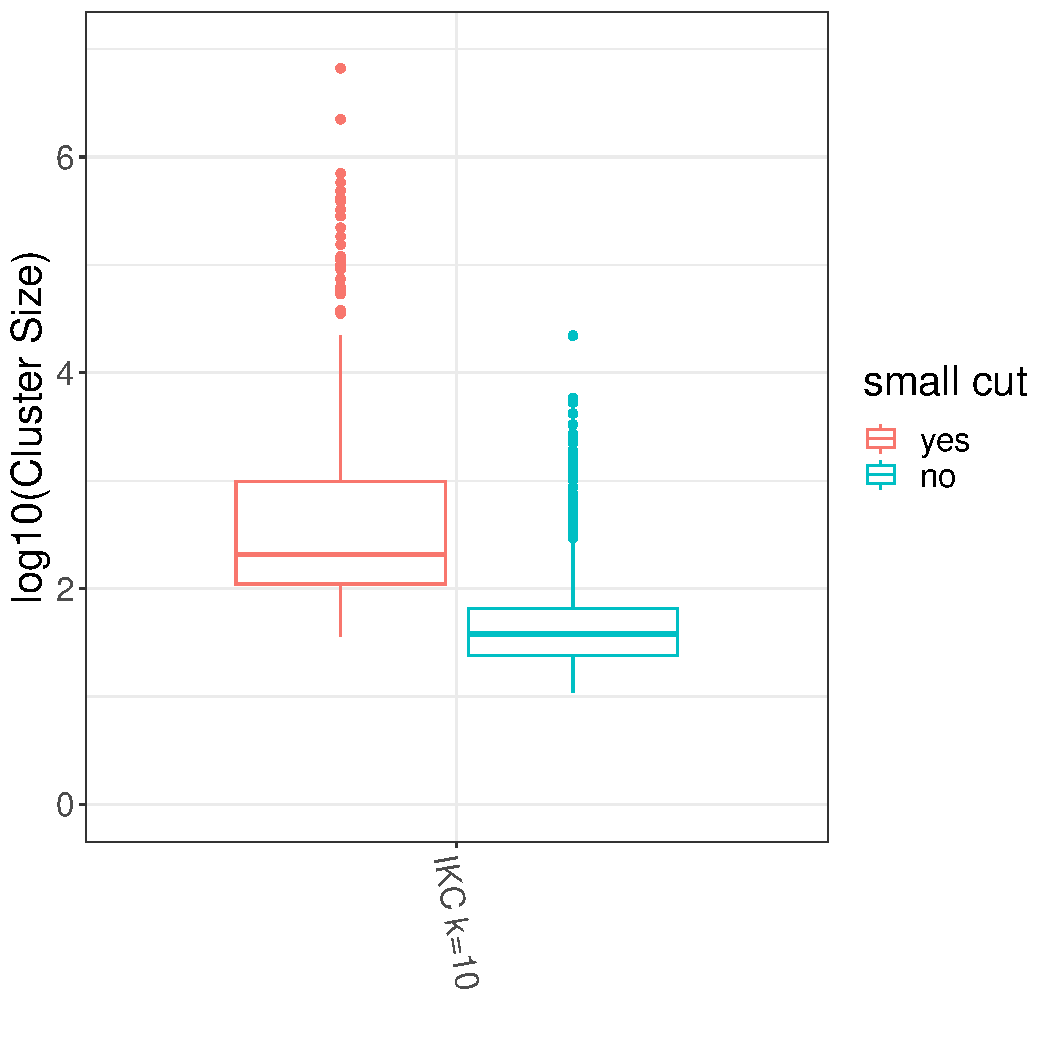
\includegraphics[width=0.37\textwidth]{figs/oc_ikc_istouched.pdf}
\caption[IKC Clusters of the Open Citations Network Impacted by CM]{\textbf{IKC Clusters of the Open Citations Network (OC) Impacted by CM}. For IKC followed by CM processing, each bar shows the total number of clusters of size at least 11. The fraction of the clusters that are affected by the CM processing (because the size of their min-cut is below the Equation \ref{eqn:our-bound} limit) is colored in red and the fraction in blue are for those that are not affected by the CM processing (because their min cut size is at least that large). Overall, 6.38\% of the input IKC clusters were modified by CM.}
\label{fig:ocistouched-ikc}
\end{figure}

\clearpage
\bibliographystyle{apalike}
\bibliography{cmv1}
\end{document}
